\chapter{线性方程组}
在初中我们已经学习了二元一次,三元一次及一些四元一次方程组的概念与解法。一次方程也叫做线性方程,一次方程组也叫做线性方程组,它是代数学中最基本、应用最广泛的内容之一。本章将进一步研究线性方程组的消元法解的
程序,引进行列式及其性质,并应用行列式理论对线性方程的求解作一般性的讨论,从而对线性方程组的理论有较系统、完整的了解。

\section{高斯消元法}
我们已经知道,解线性方程组的基本思想是消元,而且已经掌握了代入消元法和加减消元法。但这两种消元法在应用中所采取的具体步骤和顺序,往往因人而异、因题而异,尤其是在解未知数较多的线性方程组时,计算程序很麻烦,消元的顺序又不只一个途径。这就启示我们,对于任一个线性方程组,如果能有比较统一的消元程序,在解的过程中就可以充分运用现代的电子计算机,提高解题效率,也便于人们在应用中掌握。因而就有高斯消元法。

\subsection{高斯消元法}
高斯消元法实质上也是加减消元法,
只是具有明确清晰的计算程序、统一的规格,便于掌握,便于使用电子计算机。

我们先从熟悉的例子分析起。

\begin{example}
    解方程组
\begin{numcases}{}
    3x+5y=11\\ 4x-3y=5
\end{numcases}
\end{example}

\begin{solution}
$(2.1)\x \frac{1}{3}$得
\begin{numcases}{}
    x+\frac{5}{3}y=\frac{11}{3} \\
    4x-3y=5 \tag{2.2}
\end{numcases}
$(2.2)-(2.3)\x 4$得
\begin{numcases}{}
    x+\frac{5}{3}y=\frac{11}{3}  \tag{2.3} \\
    -\frac{29}{3}y=-\frac{29}{3}  
\end{numcases}
$(2.4)\x \left(-\frac{3}{29}\right)$得
\begin{numcases}{}
    x+\frac{5}{3}y=\frac{11}{3}  \tag{2.3} \\
    y=1
\end{numcases}
(2.5)代入(2.3)得:
$\begin{cases}
    x=2\\y=1
\end{cases}$
所以原方程组的解集为$\{(x,y)\}=\{(2,1)\}$。
\end{solution}


\begin{example}
    解方程组
\begin{numcases}{}
3x+y-5z=18\\
x-3y+2z=3\\
5x-11y-8z=-13    
\end{numcases}
\end{example}

\begin{solution}
先将(2.6)、(2.7)互换,得
\begin{numcases}{}
x-3y+2z=3 \tag{2.7}\\
3x+y-5z=18\tag{2.6}\\
5x-11y-8z=-13  \tag{2.8}  
\end{numcases}
$(2.6)-(2.7)\x 3$且$(2.8)-(2.7)\x 5$,得
\begin{numcases}{}
    x-3y+2z=3 \tag{2.7}\\
    16y-11z=10 \\
    4y-18z=-28   
    \end{numcases}
$(2.10)\x\frac{1}{4}$后,再与(2.9)互换,得
\begin{numcases}{}
    x-3y+2z=3 \tag{2.7}\\
    y-\frac{9}{2} z=-7 \\
    16y-11z=10  \tag{2.9}  
    \end{numcases}
$(2.9)-(2.11)\x16$后,再乘以$\frac{1}{61}$,得
\begin{numcases}{}
    x-3y+2z=3 \tag{2.7}\\
    y-\frac{9}{2} z=-7 \tag{2.11}\\
    z=2
    \end{numcases}
(2.12)代入(2.11),再代入(2.7),整理可得:
\[\begin{cases}
    x=5\\y=2\\z=2
\end{cases}\]
所以原方程组的解集为$\{(x,y,z)\}=\{(5, 2, 2)\}$。
\end{solution}

通过以上两例可以知道,解线性方程组的消元法是可按一定顺序进行的。

第一步:将$x$的系数较小的方程换到第一个,并将$x$的系数
化为1, 消去后几个方程中的$x$; 再把第二个方程中$y$的系数化为1, 消去它后边几个方程中的$y$;……直到最后一个方程中最后一个未知数的系数化为1.

第二步:将最后一个未知数的值,分别回过头代入前边各方程中去,逐步可以得出方程组的解。

以三元线性方程组为例,上面两步消元求解的过程就是:
\[\begin{cases}
    a_1x+b_1y+c_1z=d_1\\
    a_2x+b_2y+c_2z=d_2\\
    a_3x+b_3y+c_3z=d_3\\
\end{cases}\mathop{\Longrightarrow}^{\text{第一步}} \begin{cases}
    x+b'_1y+c'_1z=d'_1\\
  \qquad \quad  y+c'_2z=d'_2\\
  \qquad \qquad \quad  z=d'_3
\end{cases}\mathop{\Longrightarrow}^{\text{第二步}}  \begin{cases}
    x=d_1''\\ y=d_2''\\ z=d_3'
\end{cases}\]

在这一过程中,就是反复将方程组施行了三种基本变换:
\begin{enumerate}
    \item 互换两个方程的位置;
    \item 用一个非零常数乘以一个方程两边;
    \item 用一个非零常数乘以一个方程后,加到另一个方程上。
\end{enumerate}

必须指出,变换方程组是为了消元求解,因此,变换前后的方程组应该有相同的解集(这时我们就说这两个方程组是同解的)。那么,上述三种基本变换是否能保证方程组的同解性呢?我们肯定:经过上述三种基本变换,方程组的解集保持不变(同解的)。

对于变换1、2, 结论显然是正确的;以下以三元一次
方程组为例来证明对于变换3, 结论是正确的,我们证明方程组
\begin{equation}
    \begin{cases}
      a_1x+b_1y+c_1z=d_1\\    a_2x+b_2y+c_2z=d_2\\    a_3x+b_3y+c_3z=d_3
    \end{cases}
\end{equation}
与
\begin{equation}
    \begin{cases}
        a_1x+b_1y+c_1z=d_1\\   (a_2+ka_1)x+(b_2+kb_1)y+(c_2+kc_1)z=d_2+kd_1\\
        a_3x+b_3y+c_3z=d_3
    \end{cases} 
\end{equation}
是同解的。

\begin{proof}
    设$(\alpha,\beta,\gamma)$是(2.13)的任一个解,则应有:
\[    \begin{cases}
    a_1\alpha+b_1\beta+c_1\gamma=d_1\\   
     a_2\alpha+b_2\beta+c_2\gamma=d_2\\    
    a_3\alpha+b_3\beta+c_3\gamma=d_3
  \end{cases}\]
把第一个等式的$k$倍加到第二等式上,得
\[    \begin{cases}
    a_1\alpha+b_1\beta+c_1\gamma=d_1\\  
     (a_2+ka_1)\alpha+(b_2+kb_1)\beta+(c_2+kc_1)\gamma=d_2+kd_1\\
    a_3\alpha+b_3\beta+c_3\gamma=d_3
\end{cases} \]
这说明$(\alpha,\beta,\gamma)$也是(2.14)的一个解。用类似的方法可以证明,方程组(2.14)的任一个解也是方程组(2.13)的解,因此(2.13)与(2.14)是同解的。
\end{proof}

注意,我们讨论的只是一般情形的消元过程,还有一些特殊的情形,我们将在以后系统讨论分析。这些特殊的情形在解题中都有可能出现,需要我们灵活处理。

\begin{example}
    解方程组
    \[\begin{cases}
     \qquad \;\; 3y+2z=5\\-x+2y-3z=2\\\;\; x+4y+7z=0 
    \end{cases}\]
\end{example}


\begin{solution}
运用例2.1、例2.2相同的高斯消元法,逐步将原方程组施以三种基本变换,可得
\[\begin{split}
\text{原方程组}& \Rightarrow \begin{cases}
  \quad   x+4y+7z=0\\-x+2y-3z=2\\\qquad \;\;3y+2z=5
\end{cases} \Rightarrow \begin{cases}
    x+4y+7z=0\\\qquad  6y+4z=2\\\qquad  3y+2z=5
\end{cases}\\
&\Rightarrow \begin{cases}
    x+4y+7z=0\\\qquad \;\; y+\frac{2}{3}z=\frac{1}{3}\\\qquad \;3y+2z=5 
\end{cases}\Rightarrow \begin{cases}
    x+4y+7z=0\\\qquad \;\;y+\frac{2}{3}z=\frac{1}{3}\\\qquad \;\;\qquad  0z=4
\end{cases}
\end{split}\]

到此就会发现,方程$0\cdot z=4$无解,亦无法回代其余方程,因此,原方程组无解,或说原方程组的解集为空集$\emptyset$。
\end{solution}
    
\begin{example}
    解方程组
    \[\begin{cases}
     \qquad \;\; 3y+2z=1\\-x+2y-3z=2\\\;\; x+4y+7z=0 
    \end{cases}\]
\end{example}

\begin{solution}
    \[\begin{split}
    \text{原方程组}& \Rightarrow \begin{cases}
      \quad   x+4y+7z=0\\-x+2y-3z=2\\\qquad \;\;3y+2z=1
    \end{cases} \Rightarrow \begin{cases}
        x+4y+7z=0\\\qquad  6y+4z=1\\\qquad  3y+2z=1
    \end{cases}\\
    &\Rightarrow \begin{cases}
        x+4y+7z=0\\\qquad \;\; y+\frac{2}{3}z=\frac{1}{3}\\\qquad \;3y+2z=1 
    \end{cases}\Rightarrow \begin{cases}
        x+4y+7z=0\\\qquad \;\;y+\frac{2}{3}z=\frac{1}{3}\\\qquad \qquad  0\cdot z=0
    \end{cases}
    \end{split}\]
    
    至此可知,方程$0\cdot z=0$有无限多个解($z$可取任意实数),设$z=t$, 回代各方程中,可以得出
    \[\begin{cases}
        x=-\frac{4}{3}-\frac{13}{3}t\\
        y=\frac{1}{3}-\frac{2}{3}t\\
        z=t
    \end{cases}\]
   所以原方程组有无限多个解,其解集为
    \[\{ (x,y, z) \} = \left\{ \left(-\frac{4}{3}-\frac{13}{3}t,\; \frac{1}{3}-\frac{2}{3}t,\; t\right) \right\}, \quad t\text{为任意数}\]
 \end{solution}
    
\begin{ex}
    用高斯消元法解下列线性方程组
\begin{multicols}{2}
    \begin{enumerate}
    \item $\begin{cases}
      \quad 5x-2y=8\\-7x+10y=4 
    \end{cases}$
    \item $\begin{cases}
        2x-3y+4z=8\\ 5x-y-8z=-21\\3x+5y-7z=-8
    \end{cases}$
    \item $\begin{cases}
      \qquad   y+2z=4\\x-3y\qquad =-8\\4x\quad\;\;\; -5z=7
    \end{cases}$
    \item $\begin{cases}
        7x-y+2z=1\\\qquad 5y-3z=0\\14x-2y+4z=1
    \end{cases}$
    \item $\begin{cases}
        3x-7y\qquad =2\\\qquad\quad  y-z=1\\12x-28y\quad =8
    \end{cases}$
\end{enumerate}    
\end{multicols}
\end{ex}
    
\subsection{一般二元一次方程组解的公式讨论}

利用高斯消元
法,我们对一般的二元一次方程组
\begin{numcases}{(\rm I)}
    a_1x+b_1y=c_1\\
    a_2x+b_2y=c_2
\end{numcases}
求解,并讨论它的各种情形。

在方程组(I)中,我们假定$a_1$与$b_1$, $a_2$与$b_2$, $a_1$与$a_2$,$b_1$与$b_2$分别不同时为零,因为,如若不然,不论上述哪一种
情形发生,方程组的解将是容易讨论的,同学们不妨试着自行讨论一下。

在这个假定下,利用高斯消元法(假定$a_1\ne 0$),可得
\begin{numcases}{}
x+\frac{b_1}{a_1}y=\frac{c_1}{a_1}\\
\frac{a_1b_2-a_2b_1}{a_1}y=\frac{a_1c_2-a_2c_1}{a_1}    
\end{numcases}
再将(2.18)变形后,可得
\begin{numcases}{}
    x+\frac{b_1}{a_1}y=\frac{c_1}{a_1} \tag{2.17}\\
    (a_1b_2-a_2b_1)y=a_1c_2-a_2c_1    
    \end{numcases}
由方程出发,可分别讨论如下:
\begin{enumerate}
    \item 当$a_1b_2-a_2b_1\ne 0$时,由(2.19)并代入(2.17)可以
得出方程组(I)唯一的一个解
\[\begin{cases}
    x=\frac{c_1b_2-c_2b_1}{a_1b_2-a_2b_1}   \\
    y=\frac{a_1c_2-a_2c_1 }{a_1b_2-a_2b_1}
\end{cases}\]
这就是原方程组的解的公式。

\item 当$a_1b_2-a_2b_1=0$时,由(2.19)又可以分为两种情形
讨论:
\begin{enumerate}
    \item 若$a_1c_2-a_2c_1\ne 0$,方程(2.19)变为一个矛盾方
程,共解集是空集,因而原方程组也就无解,其解集仍是空集。
\item 若$a_1c_2-a_2c_1=0$, 则方程(2.19)变为:$0y=0$, $y$可取任意实数$t$, 代入(2.17)得:
\[x=\frac{c_1}{a_1}-\frac{b_1}{a_1}t\]
这时方程组(I)有无限多解,解集为
\[\{(x,y)\}=\left\{\left(\frac{c_1-b_1t}{a_1}\right),\quad \text{$t$ 为任意实数}\right\}\]
\end{enumerate}
\end{enumerate}

\begin{blk}{定理}
方程组$\begin{cases}
    a_1x+b_1y=c_1\\
    a_2x+b_2y=c_2
\end{cases}$
其中$a_1$与$b_1$, $a_2$与$b_2$, $b_1$与$b_2$分别不同时为零。
\begin{enumerate}
    \item 当$a_1b_2-a_2b_1\ne 0$,它有唯一解;
    \[x=\frac{c_1b_2-c_2b_1}{a_1b_2-a_2b_1} ,\qquad 
    y=\frac{a_1c_2-a_2c_1 }{a_1b_2-a_2b_1}\]
    \item 当$a_1b_2-a_2b_1= 0$,且$a_1c_2-a_2c_1\ne 0$(或$c_1b_2-c_1b_1\ne 0$),它无解;
    \item 当$a_1b_2-a_2b_1= 0$,且$a_1c_2-a_2c_1= 0$,$c_1b_2-c_1b_1=0$,它有无限多个解。
\end{enumerate}
\end{blk}

\begin{example}
讨论方程组
\[\begin{cases}
    (a-b) x+ (a+b) y=2 (a^2-b^2)\\
    (a+b) x+ (a-b)y=2 (a^2+b^2)
\end{cases}\]
的解的情况。    
\end{example}

\begin{solution}
设$$a_1=a-b,\quad b_1 =a+b,\quad c_1=2 (a^2-b^2)$$
$$a_2=a+b,\quad b_2 =a-b,\quad c_2=2 (a^2+b^2)$$
则$$a_1b_2-a_2b_1=-4ab,\; a_1c_2-a_2c_1=-4ab(a-b),\; b_2c_1-b_1c_2=-4ab(a+b)$$所以
\begin{enumerate}
\item 若$a\ne 0$且$b\ne 0$, 则方程组有唯一解:
\[x=a+b,\qquad y=a-b\]
\item 若$a=0$或$b=0$, 则方程组有无限多个解。
\begin{enumerate}
    \item 在$a=0$, $b\ne 0$时,方程组的解集为:
\[\{(x,y)\}=\{(2b+t,t)|\text{$t$为任意数}\}\]
\item 在$a=0$, $b=0$时,方程组解集为
\[\{(x,y)\}=\{(2a-t,t)|\text{$t$为任意数}\}\]
\end{enumerate}

\item 若$a=b=0$, 则原方程组成为:
\[\begin{cases}
    0x+0y=0 \\ 0x+0y=0 
\end{cases}\]
显然两个方程组都是恒等式,$x,y$都可取任何数,因此方程组的解集是:
\[\{(x,y)\} =\{ (s,t)|\text{$s,t$为任意数}\}\]
\end{enumerate}
注意:本题不存在无解的情况。
\end{solution}

\begin{example}
有一个三位数,已知其十位数字等于其个位数字与百位数字之和,其个位数字与十位数字之和为$a$, 如果把三个数字的顺序倒过来,则所得新的三位数比原三位数大99. 求原三位数,并问参数$a$可取哪些值?
\end{example}


\begin{solution}
设原三位数的个位字为$x$, 百位数字为$y$, 由题目可知十位数字就是$a-x$. (其中$x,y$都是$1, 2,\ldots,9$这几个数字之一;$a-x$是$0, 1,\ldots,9$这十个数字之一)。显然,$3\le a\le 18$. 依题意有:
\[\begin{cases}
    x+y=a-x\\
    100x+10(a-x)+y=100y+10(a-x)+x+99
\end{cases}\]
将上述方程组变换为:
\[\begin{cases}
    2x+y=a\\x-y=1
\end{cases}\]
由消元法可得出:$\begin{cases}
    x=\frac{1}{3}(a+1)\\ y=x-1
\end{cases}$
由上面这两个等式,不难断定:$a+1$须是3的倍数。所以,$a$只可能取$5, 8, 11, 14, 17$之中的一个值,直接计算可得:
\begin{itemize}
    \item $a=5$时,则$x=2$, $y=1$, $a-x=8$,
    可得出所求三位数为232;
\item $a=8$时,则$x=3$, $y=2$, $a-x=5$,
可得出所求三位数为253;
\item $a=11$时,则$x=4$, $y=8$, $a-x=7$,
可得出所求三位数为374;
\item $a=14$时,则$x=5$, $y=4$, $a-x=9$,
可得出所求三位数为495,
\item $a=17$时,虽可求出$x=6$, $y=5$, 但$a-x=11$已不符
合题意,因此,这种情形不可能出现。
 \end{itemize}   

所以,参数$a$分别取值5, 8, 11,与14,相应的三位数为:132, 253, 374, 495.
\end{solution}    

\begin{ex}
    试判别和讨论下列线性方程组的解的情形。
    \begin{multicols}{2}
\begin{enumerate}
    \item $\begin{cases}
        3x-5y=20\\6x-10y=15
    \end{cases}$
    \item $\begin{cases}
        3x-y=8\\2x+ay=7
    \end{cases}$
    \item $\begin{cases}
mx+y=m+1\\x+my=2m        
    \end{cases}$
\end{enumerate}        
    \end{multicols}
\end{ex}

\section*{习题2.1}
\addcontentsline{toc}{subsection}{习题2.1}

\begin{enumerate}
    \item 用高斯消元法解下列方程组:
\begin{multicols}{2}
\begin{enumerate}
    \item $\begin{cases}
        2x+8y-5z=3\\x-2y+z=0\\x+y+3z=7
    \end{cases}$
    \item $\begin{cases}
        x+y+2z=4\\2x-y+3z=4\\x+y+2z=3
    \end{cases}$
    \item $\begin{cases}
         x+2y-8z=5\\8x-2y+z=4\\-3x-6y+9z=15
    \end{cases}$
    \item $\begin{cases}
         x+2y-3z=5\\ -2x-4y+6z=-10\\ \frac{1}{2}x+y-\frac{3}{2}z=\frac{5}{2}
    \end{cases}$
    \item $\begin{cases}
        x_1+8x_2+5x_3+7x_4=12\\ 8x_1+5x_2+7x_3+x_4 =0\\
    5x_1+7x_2+x_3+3x_4=4\\ 7x_1+x_2+3x_3+5x_4=16
    \end{cases}$
    
\end{enumerate}    
\end{multicols}

    \item 讨论下列各方程组的解的情况:
\begin{multicols}{2}
\begin{enumerate}    
    \item $\begin{cases}
      x+y=12\\ x+ay=4  
    \end{cases}$
    \item $\begin{cases}
        6x-5y=25\\4x+ay=b
    \end{cases}$
    \item $\begin{cases}
        x=by\\px=qy
    \end{cases}$
    \item $\begin{cases}
        ax+by=a^2+2a+b^2\\
        bx+ay=a^2+2b+b^2
    \end{cases}$
\end{enumerate}    
\end{multicols}
    \item 一个两位数的两数字之和为 $a$, 若颠倒这两个数字的顺序,所得新的两位数比原数小36, 问$a$可能取那些值?原来的两位数是什么?
    \item 试判断$m$取何值时,下列方程组有唯一解:
\begin{enumerate}
    \item $\begin{cases}
        (m-1)x-(m+1)y=m+1\\ m^2x-(m+1)y=m-1
    \end{cases}$
    \item $\begin{cases}
x-(m^2-5)y=-1\\ (m+1)x -(m+1)^2y=1       
    \end{cases}$
\end{enumerate}

\item  高斯消元法对方程组的三种基本变换中,若把变换改为“用任一个常数乘一个方程。”删去“非零”二字行吗?为
什么?举例说明。
\end{enumerate}

\section{二阶行列式与二元线性方程组}
本节我们将从二元线性方程组的解的公式入手,引进二阶行列式的概念,从而学习二元线性方程组的行列式解法,并应用行列式讨论它的解的各种情形。

\subsection{二阶行列式}

一般的二元线性方程组
\begin{numcases}{(\text{I})}
    a_1x+b_1y=c_1\\
    a_2x+b_2y=c_2
\end{numcases}
当$a_1b_2-a_2b_1\ne 0$时,有唯一解,即
\begin{equation}
\begin{cases}
    x=\frac{c_1b_2-c_2b_1}{a_1b_2-a_2b_1}\\
    y=\frac{a_1c_2-a_2c_1}{a_1b_2-a_2b_1}
\end{cases}    
\end{equation}

分析公式(2.22)可以看出,两个分母都是$a_1b_2-a_2b_1$, 其中只含有未知数的系数。如果把方程组(I)中未知数的系数分离出来,按照它们原有的位置排列成一个正方形,即
\begin{center}\Large
    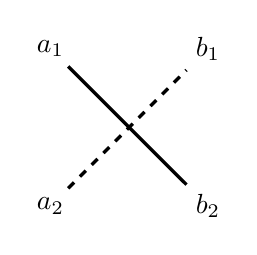
\begin{tikzpicture}
\node (A1) at (-1,1){$a_1$};
\node (A2) at (-1,-1){$a_2$};
\node (B1) at (1,1){$b_1$};
\node (B2) at (1,-1){$b_2$};
\draw [very thick](A1)--(B2);
\draw[dashed, very thick] (A2)--(B1);
    \end{tikzpicture}
\end{center}
那么可以看到$a_1b_2-a_2b_1$是这样两项的和:一项是正方形中实线所示的对角线(称为主对角线)上两个数的积,取正号;另一项是正方形中虚线所示的对角线(称为副对角线)上两个数的积,取负号。

为了便于记忆,我们将排正方形的四个数的两侧各加一
条竖直线,表示成
\[\begin{vmatrix}
    a_1&b_1\\a_2&b_2
\end{vmatrix}\]
并规定这个符号就是$a_1b_2-a_2b_1$即:
\begin{equation}
    \begin{vmatrix}
        a_1&b_1\\a_2&b_2
    \end{vmatrix}=a_1b_2-a_2b_1
\end{equation}

这时,(2.23)式的左边,就叫做二阶行列式;而(2.23)式的右边就是二阶行列式的展开式。

二阶列行式中,四个数称为它的元素;四个元素排成两
横排(称为行)两竖排(称为列),因而二阶行列共有二行二列。

所以,二阶行列式是一个值,它可按照(2.23)用对角线法则展开并计算出来。

\begin{example}
    展开并计算下列行列式:
\begin{multicols}{2}
\begin{enumerate}
    \item $\begin{vmatrix}
        2&3\\-5&-8
    \end{vmatrix}$
    \item $\begin{vmatrix}
        0&-7\\-3&10
    \end{vmatrix}$
    \item $\begin{vmatrix}
        m+1&m+2\\m&m+1
    \end{vmatrix}$
    \item $\begin{vmatrix}
        \sin x& \cos x\\ \cos x&\sin x
    \end{vmatrix}$
\end{enumerate}
\end{multicols}
\end{example}

\begin{solution}
由对角线法则可得,  
\begin{enumerate}
    \item $\begin{vmatrix}
        2&3\\-5&-8
    \end{vmatrix}=2\x(-8)-3\x (-5)=-1$
    \item $\begin{vmatrix}
        0&-7\\-3&10
    \end{vmatrix}=-21$
    \item $\begin{vmatrix}
        m+1&m+2\\m&m+1
    \end{vmatrix}=(m+1)^2-m(m+2)=1$
    \item $\begin{vmatrix}
        \sin x& \cos x\\ \cos x&\sin x
    \end{vmatrix}=\sin^2x-\cos^2x=-\cos2x$
\end{enumerate}
\end{solution}
  
\begin{ex}
\begin{enumerate}
    \item 展开并计算下列行列式的值:
\begin{multicols}{2}
\begin{enumerate}
    \item $\begin{vmatrix}
    8&4\\3&9
\end{vmatrix}$
    \item $\begin{vmatrix}
    a&a^2\\b&b^2
\end{vmatrix}$
\item $\begin{vmatrix}
    -3&21\\-1&7
\end{vmatrix}$
\item $\begin{vmatrix}
    6a-b&2b\\3a&b
\end{vmatrix}$
\item $\begin{vmatrix}
    \log_a x&\log_a x\\m&n
\end{vmatrix}$
\item $\begin{vmatrix}
    \sin x&\tan x\\ \cos x&\cot x
\end{vmatrix}$
\item $\begin{vmatrix}
     1-\sqrt{2}&2-\sqrt{3}\\2+\sqrt{3}&1+\sqrt{2}
\end{vmatrix}$
\item $\begin{vmatrix}
     x-1&x^3\\1&x^2+x+1
\end{vmatrix}$
\end{enumerate}
\end{multicols}

    \item 试试看,你能把下列各式分别用几个二阶行列式表示出来吗?
    \[am-bn,\qquad am+bn,\qquad a_1b_2-a_2b_1\]
    \item 求证:
    $\begin{vmatrix}
        a_1+ka_2 &b_1+kb_2 \\ a_2&b_2
    \end{vmatrix}=\begin{vmatrix}
        a_1  &b_1  \\ a_2&b_2
    \end{vmatrix}$
\end{enumerate}
\end{ex}

\subsection{二元线性方程组解的行列式表示及讨论}

在二元线性方程组的解的公式中,仔细观察可以发现,两分母,分子都可以很有规律地用行列式表示出来,即
\[\begin{split}
    a_1b_2-a_2b_1&=\begin{vmatrix}
        a_1&b_1\\a_2&b_2
    \end{vmatrix}\\
    c_1b_2-c_2b_1&=\begin{vmatrix}
        c_1&b_1\\c_2&b_2
    \end{vmatrix}\\
    a_1c_2-a_2c_1&=\begin{vmatrix}
        a_1&c_1\\a_2&c_2
    \end{vmatrix} 
\end{split}\]
这样,二元线性方程组解的公式就可以表示为:

当$\begin{vmatrix}
    a_1&b_1\\a_2&b_2
\end{vmatrix}\ne 0$时,
\[x=\frac{\begin{vmatrix}
    c_1&b_1\\c_2&b_2
\end{vmatrix}}{\begin{vmatrix}
    a_1&b_1\\a_2&b_2
\end{vmatrix}},\qquad y=\frac{\begin{vmatrix}
    a_1&c_1\\a_2&c_2
\end{vmatrix}}{\begin{vmatrix}
    a_1&b_1\\a_2&b_2
\end{vmatrix}}\]
为简便起见,通常把上述三个二阶行列式分别记为
\[D=\begin{vmatrix}
    a_1&b_1\\a_2&b_2
\end{vmatrix},\qquad D_x=\begin{vmatrix}
    c_1&b_1\\c_2&b_2
\end{vmatrix},\qquad D_y=\begin{vmatrix}
    a_1&c_1\\a_2&c_2
\end{vmatrix}\]
其中$D$ 的元素由方程组的未知数系数按顺序组成,就叫做这个方程组的系数行列式;$D_x$的元素由$D$将第一列元素($x$的系数)分别换成相应的常数项组成;$D_y$的元素由$D$将第二列元素($y$的系数)分别换成相应的常数项组成。

这样二元线性方程组(I)的解的公式,就可简化为:当$D\ne 0$时,
\[\begin{cases}
    x=\frac{D_x}{D}\\y=\frac{D_y}{D}
\end{cases}\]
即:二元线性方程组(I)的解集为
\[\{(x,y)\}=\left\{\left(\frac{D_x}{D},\; \frac{D_y}{D}\right)\right\}\]

\begin{example}
    用行列式法解方程组
    $\begin{cases}
11x-2y+5=0\\
8x+7y+24=0        
    \end{cases}$
\end{example}

\begin{solution}
    先将所给方程组写为一般形式
\[\begin{cases}
    11x-2y=-5\\
    8x+7y=-24
\end{cases}\]
再计算行列式$D$, $D_x$, $D_y$:
\[D=\begin{vmatrix}
    11&-2\\3&7
\end{vmatrix}=83\ne 0,\quad  D_x=\begin{vmatrix}
    -5&-2\\-24&7
\end{vmatrix}=-83,\quad  D_y=\begin{vmatrix}
    11&-5\\3&-24
\end{vmatrix}=-249\]
根据解的公式,得
\[x=\frac{D_x}{D}=-1,\qquad y=\frac{D_y}{D}=-3\]
所以,原方程组的解集为$\{(x,y)\}=\{(-1,-3)\}$。
\end{solution}

在使用行列式方法解二元线性方程组时,如果出现$D=0$时,解的公式不适用,这时可以仿照前文中对方程组解的讨论,得到以下结论:
\begin{itemize}
    \item 当$D=0$, 且$D_x\ne 0$(或$D_y\ne 0$)时,方程组的解集是空集$\emptyset$;
    \item 当$D=0$, 且$D_x=D_y=0$时,方程组有无限多个解,它的解集可引进一个参数表示。
\end{itemize}

注意,我们这里所指的二元线性方程组,限定其中的
$a_1$与$a_2$,$a_1$与$b_1$,$a_2$与$b_2$,$b_1$与$b_2$不同时为0。

\begin{example}
    用行列式法解下列方程组,并讨论:
    \[\begin{cases}
        mx+y-m-1=0\\
        x+my-2m=0   
    \end{cases}\]
   \end{example}
   
   
   
   \begin{solution}
先将原方程化为一般形式:
\[\begin{cases}
    mx+y=m+1\\
    x+my=2m   
\end{cases}\]
再计算各行列式:
\[\begin{split}
D&=\begin{vmatrix}
    m&1\\1&m
\end{vmatrix}=m^2-1=(m+1)(m-1)\\
D_x&=\begin{vmatrix}
    m+1&1\\2m&m
\end{vmatrix}=m(m+1)-2m=m(m-1)\\
D_y&=\begin{vmatrix}
    m&m+1\\1&2m
\end{vmatrix}=2m^2-(m+1)=(2m+1)(m-1)
\end{split}\]
所以
\begin{itemize}
    \item 当$m\ne -1$, $m\ne 1$时,$D\ne 0$方程组有唯一解,它的解集为
\[\{ (x,y) \} = \left\{ \left(\frac{m}{m+1},\frac{2m+1}{m+1}\right) \right\}\]
\item 当$m=-1$时,$D=0$, $D_x\ne 0$, 方程组无解,它的解集为$\emptyset$。
\item 当$m=1$时,$D=D_x=D_y=0$方程组有无限多个解,这时由于原方程组变为
$\begin{cases}
    x+y=2\\x+y=2
\end{cases}$
实际上就是$x+y=2$, 若令$x=t$, 则$y=2-t$, 因此,方程组的解集可表示为:
\[\{(x,y)\}=\{(t,2-t)|\text{$t$为任意数}\}\]
\end{itemize}

注意,在上述参数表示法中,可以有不同的表示法,如若令$y=a$, 则$x=2-a$, 解集就应表示为$\{(x,y)\}=\{(2-a,a)|\text{$a$为任意数}\}$。
\end{solution}

\begin{ex}
\begin{enumerate}
    \item 用行列式法解下列方程组
\begin{enumerate}
    \item $\begin{cases}
        x-8y=10\\6x-7y-11=0
    \end{cases}$
    \item $\begin{cases}
        14b-6y=-1\\ 3x+7y-6=0   
    \end{cases}$
    \item $\begin{cases}
        mx+ny=1\\nx+my=-1,\quad  (m\ne n) 
    \end{cases}$
    \item $\begin{cases}
        x\cos A-y\sin A=\cos B\\ x\sin A+y\cos A=\sin B
    \end{cases}$
\end{enumerate}

    \item 解下列方程组,并讨论
\begin{enumerate}
    \item $\begin{cases}
        x+ (m-1)y=1\\(m-1) x+y=2
    \end{cases}$
    \item $\begin{cases}
        mx+y=1\\ 4x+my-m=0
    \end{cases}$
    \item $\begin{cases}
        kx+ (2a-1) y=a^2+2a-1\\ x+ay=2a
    \end{cases}$
\end{enumerate}
\end{enumerate}   
\end{ex}

\section*{习题2.2}
\addcontentsline{toc}{subsection}{习题2.2}
\begin{enumerate}
    \item 计算下列行列式的值
\[\begin{vmatrix}
    \sqrt{6}&\sqrt{4}\\\sqrt{2}&\sqrt{3}
\end{vmatrix},\qquad \begin{vmatrix}
    \log_a b&4\\ 3& \log_b a
\end{vmatrix},\qquad\begin{vmatrix}
    e^{x+y}&e^x-1\\e^x+1&e^{x-y}
\end{vmatrix},\qquad\begin{vmatrix}
    1&1\\-\tan^2\alpha&1
\end{vmatrix}\]

\item 求证:
\begin{enumerate}
    \begin{multicols}{2}
    \item $\begin{vmatrix}
        a_1&b_1\\a_2&b_2
    \end{vmatrix}=\begin{vmatrix}
        a_1&a_2\\b_1&b_2
    \end{vmatrix}$
    \item $\begin{vmatrix}
        b_1 & b_2 \\a_1 &a_2
    \end{vmatrix}=-\begin{vmatrix}
        a_1&b_1\\a_2&b_2
    \end{vmatrix}$   
    \item $\begin{vmatrix}
        ka_1&kb_1\\b_1&a_2
    \end{vmatrix}=k\begin{vmatrix}
        a_1&b_1\\a_2&b_2
    \end{vmatrix}$
    \item $\begin{vmatrix}
        ka_1&\ell a_1\\ka_2& \ell a_2
    \end{vmatrix}=0$
\end{multicols}
    \item $\begin{vmatrix}
        a_1+a' &b_1+b'\\a_2&b_2
    \end{vmatrix}=\begin{vmatrix}
        a_1&b_1 \\a_2&b_2
    \end{vmatrix}+\begin{vmatrix}
        a'&b'\\ a_2&b_2
    \end{vmatrix}$
\end{enumerate} 

\item 用行列式解下列方程组:
\begin{multicols}{2}
\begin{enumerate}
    \item $\begin{cases}
        13x-7y-10=0\\19x+15y-2=0
    \end{cases}$
    \item $\begin{cases}
        \frac{7}{m}+\frac{9}{n}=3\\
        \frac{17}{m}+\frac{7}{n}=5
    \end{cases}$
\end{enumerate}
\end{multicols}
\item 解下列关于$x,y$的方程组,并讨论。
\begin{multicols}{2}
\begin{enumerate}
    \item $\begin{cases}
        mx+y=2m+1\\x-my=2-m
    \end{cases}$
    \item $\begin{cases}
        mx+y=-1\\8mx-my=2m+3
    \end{cases}$
    \item $\begin{cases}
        (a-1)x-(a^2-1)y=1\\
        (a^2-1)x+(a-1)y=2
    \end{cases}$
    \item $\begin{cases}
        kx+y=k+1\\
        x+ky=2k
    \end{cases}$
\end{enumerate}    
\end{multicols}

\item 当$k$为何值时,方程组$\begin{cases}
    4x+3y=1\\kx+(k-2)y=3
\end{cases}$的解中,$x$与$y$的值取异号?
\end{enumerate}

\section{三阶行列式与三元线性方程组}
\subsection{三阶行列式}

仿照二阶行列式,我们可以把九个数排成三行三列的正方形,并在两侧各加一竖直线。如
\begin{equation}
    \begin{vmatrix}
  a_1&b_1&c_1\\a_2&b_2&c_2\\a_3&b_3&c_3\\      
    \end{vmatrix}
\end{equation}
并规定它表示一个数
\begin{equation}
    a_1b_2c_3+a_2b_3c_1+a_3b_1c_2-a_3b_2c_1-a_2b_1c_3-a_1b_3c_2
\end{equation}

这时我们就把(2.24)叫做一个三阶行列式,(2.25)式就叫做这个三阶行列式的展开式(或这三阶行列式的值。)

三阶行列式共有九个元素,它的值也可以按上右图所示
的对角线法则计算出来:

实线所连三元素的乘积都取正号,共三项;虚线所连三元素乘积,都取负号,共三项。

\begin{example}
    用对角线法则计算下列三阶行列式:
\begin{multicols}{3}
\begin{enumerate}
    \item $\begin{vmatrix}
        1&3&5\\2&4&8\\3&0&-1
    \end{vmatrix}$
    \item $\begin{vmatrix}
        2&-3&1\\4&-1&7\\-1&5&2
    \end{vmatrix}$
    \item $\begin{vmatrix}
        x&y&z\\z&x&y\\y&z&x
    \end{vmatrix}$
\end{enumerate} 
\end{multicols}
\end{example}

\begin{solution}
由对角线法则可得:
\[\begin{split}
    \begin{vmatrix}
        1&3&5\\2&4&8\\3&0&-1
    \end{vmatrix}&=1\cdot 4\cdot (-1)+2\cdot 0\cdot 5+3\cdot 3\cdot8-3\cdot4\cdot5-2\cdot 3\cdot (-1)-1\cdot 0\cdot 8\\
    &=-4+0+77-60+6-0=14
\end{split}\]
\[\begin{split}
    \begin{vmatrix}
        2&-3&1\\4&-1&7\\-1&5&2
    \end{vmatrix}&=2\cdot(-1)\cdot2+4\cdot5\cdot1+(-1)\cdot(-3)\cdot7-(-1)\cdot(-1)\cdot1-4\cdot(-3)\cdot2-2\cdot5\cdot7\\
    &=-4+20+21-1+24-70=-10
\end{split}\]
\[\begin{vmatrix}
    x&y&z\\z&x&y\\y&z&x
\end{vmatrix}=x^3+y^3+z^3-3xyz\]
\end{solution}

\begin{ex}
\begin{enumerate}
\item 计算下列三阶行列式    
\[\begin{vmatrix}
    3&1&2\\1&0&0\\-1&0&0
\end{vmatrix},\quad \begin{vmatrix}
    1&a&a^2\\1&b&b^2\\1&c&c^2
\end{vmatrix},\quad \begin{vmatrix}
    0&a&b\\a&0&c\\b&c&0
\end{vmatrix},\quad \begin{vmatrix}
    1&a&b\\-a&1&c\\-b&-c&1
\end{vmatrix},\quad \begin{vmatrix}
    a&d&e\\0&b&d\\0&0&c
\end{vmatrix}\]

\item 先计算行列式的值,再比较结果找出各组中两行列式之间的关系:
\begin{enumerate}
    \item $\begin{vmatrix}
        1&4&7\\2&5&8\\3&6&9
    \end{vmatrix},\qquad \begin{vmatrix}
        1&2&3\\4&5&6\\7&8&9
    \end{vmatrix}$
    \item $\begin{vmatrix}
        a&1&2\\1&a&1\\2&1&a
    \end{vmatrix},\qquad \begin{vmatrix}
        ak&k&2k\\1&a&1\\2&1&a
    \end{vmatrix}$
\end{enumerate}
\end{enumerate}    
\end{ex}

\subsection{三阶行列式的性质}

为了简化行列式的计算,更好地掌握这一工具,我们进一步学习行列式的性质。

\begin{blk}{定理1 }
    如果把一个行列式的每一行(列),同时改为同号数的列(行),那么,所得的行列式与原行列式的值相等。
\[\Delta=\begin{vmatrix}
    a_1&b_1&c_1\\a_2&b_2&c_2\\a_3&b_3&c_3
\end{vmatrix}=\begin{vmatrix}
    a_1&a_2&a_3\\b_1&b_2&b_3\\c_1&c_2&c_3
\end{vmatrix}=\Delta'\]
\end{blk}

 \begin{proof}
由对角线法则知    
\[\begin{split}
    \Delta &=a_1b_2c_3+a_2b_3c_1+a_3b_1c_2-a_3b_2c_1-a_2b_1c_3-a_1b_3c_2\\
    \Delta'&=a_1b_2c_3+a_2b_3c_1+a_3b_1c_2-a_3b_2c_1-a_2b_1c_3-a_1b_3c_2\\
\end{split}\]
所以$\Delta=\Delta'$
 \end{proof}


 由定理1可知:对于行列式的行成立的性质对于列也一定成立;反过来,对于列成立的性质对于行也一定成立,所以今后关于行列式的性质,只需对行证明就行了。

\begin{blk}{定理2}
    如果把一个行列式的任意两行(列)对调,那么,所得的行列式与原行列式的绝对值相等,符号相反。
    \[\Delta=\begin{vmatrix}
        a_1&b_1&c_1\\a_2&b_2&c_2\\a_3&b_3&c_3
    \end{vmatrix}=-\begin{vmatrix}
        a_2&b_2&c_2\\a_1&b_1&c_1\\a_3&b_3&c_3
    \end{vmatrix}=-\Delta'\]
\end{blk} 

\begin{proof}
    只要以对调第一、二行为例证明结论,其它行(列)对调的证明是类似的。
    仍由三阶行列式的对角线法则可得
    \[\begin{split}
        \Delta&=a_1b_2c_3+a_2b_3c_1+a_3b_1c_2-a_3b_2c_1-a_2b_1c_3-a_1b_3c_2\\
        &=-(a_2b_1c_3+a_1b_3c_2+a_3b_2c_1-a_3b_1c_2-a_1b_2c_3-a_2b_3c_1)\\
        &=-\Delta'
    \end{split}\]
    所以$\Delta=-\Delta'$
\end{proof}

\begin{blk}{定理3}
 如果一个行列式中,有两行(列)元素完全对应相同,那么,这个行列式的值必须等于零。   
 \[\Delta=\begin{vmatrix}
     a_1&a_2&a_3\\ b_1&b_2&b_3\\a_1&a_2&a_3
 \end{vmatrix}=0\]
\end{blk}

\begin{proof}
只要将行列式中相同的两行(列)对调,则所得行列式仍为$-\Delta$, 但根据定理2又可知,对调后应得$-\Delta$。于是就有,    
\[\Delta=-\Delta\]
所以可得:$\Delta=0$。
\end{proof}

\begin{blk}{定理4}
如果把一个行列式的某一行(列)的所有元素同乘以任一数$k$, 那么,所得行列式的值就等于原行列式值的$k$倍。
\[\Delta'=\begin{vmatrix}
    a_1&b_1&c_1\\ka_2&kb_2&kc_2\\a_3&b_3&c_3
\end{vmatrix}=k\cdot \begin{vmatrix}
    a_1&b_1&c_1\\a_2&b_2&c_2\\a_3&b_3&c_3
\end{vmatrix}=k\Delta\]
\end{blk}

\begin{proof}
由对角线法则将它们展开、比较,就可直接证明结论$\Delta'=k\Delta$是正确的。
\end{proof}

\begin{blk}{定理5}
    如果在行列式中,某一行(列)各元素有公因子时,则可以把公因子提到行列式的外边。
\[\begin{vmatrix}
    ka_1&kb_1&kc_1\\a_2&b_2&c_2\\a_3&b_3&c_3
\end{vmatrix}=k\cdot \begin{vmatrix}
    a_1&b_1&c_1\\a_2&b_2&c_2\\a_3&b_3&c_3
\end{vmatrix}
    \]
\end{blk}

这定理的证明可由定理4直接得出,这里不再重述,但要指出,这个定理可以使行列式计算简化,在应用中很重要。例如,运用它可这样计算行列式:
\[\begin{split}
\begin{vmatrix}
    -\tfrac{1}{2}&-\tfrac{2}{3}&-1\\
    \tfrac{5}{2}&\tfrac{4}{3}&0\\
    \tfrac{9}{2}&\tfrac{7}{3}&1
\end{vmatrix}&=(-1)\x\frac{1}{2}\x\frac{1}{3}\x\begin{vmatrix}
    1&2&1\\5&4&0\\9&7&1
\end{vmatrix}\\
&=\left(-\frac{1}{6}\right)\x(-7)=1\frac{1}{6}
\end{split}\]

\begin{blk}{定理6}
    如果一个行列式中有一行(列)的元素全为零,则这个行列式的值等于零。
    \[\begin{vmatrix}
        0&0&0\\a_2&b_2&c_2\\a_3&b_3&c_3
    \end{vmatrix}=0\]
\end{blk}

\begin{proof}
    由定理5与零的运算特性可得
\[\begin{vmatrix}
    0&0&0\\a_2&b_2&c_2\\a_3&b_3&c_3
\end{vmatrix}=\begin{vmatrix}
    0\cdot a_1&0\cdot b_1&0\cdot c_1\\a_2&b_2&c_2\\a_3&b_3&c_3
\end{vmatrix}=0\cdot\begin{vmatrix}
    a_1&b_1&c_1\\a_2&b_2&c_2\\a_3&b_3&c_3
\end{vmatrix}=0\]
\end{proof}

\begin{blk}{定理7}
    如果一个行列式中有两行(或两列)的对应元素成比例,则这个行列式等于零。
\[\begin{vmatrix}
    ka_2&kb_2&kc_2\\a_2&b_2&c_2\\a_3&b_3&c_3
\end{vmatrix}=0\]
\end{blk}

\begin{proof}
    由定理5及定理8可以知道:
    \[\begin{vmatrix}
        ka_2&kb_2&kc_2\\a_2&b_2&c_2\\a_3&b_3&c_3
    \end{vmatrix}=k\cdot\begin{vmatrix}
        a_2&b_2&c_2\\a_2&b_2&c_2\\a_3&b_3&c_3
    \end{vmatrix}=k\cdot 0=0\]
\end{proof}

\begin{blk}{定理8}
如果行列式某一行(或一列)的元素都是二项式之和的形式,则这个行列式等于两个行列式之和。
\[\begin{vmatrix}
    a_1+a'_1&b_1+b'_1&c_1+c'_1\\a_2&b_2&c_2\\a_3&b_3&c_3
\end{vmatrix}=\begin{vmatrix}
    a_1&b_1&c_1\\a_2&b_2&c_2\\a_3&b_3&c_3
\end{vmatrix}+\begin{vmatrix}
    a'_1&b'_1&c'_1\\a_2&b_2&c_2\\a_3&b_3&c_3
\end{vmatrix}\]
\end{blk}

证明要点:用三阶行列式的对角线法则,将左边的行列式展开,再由乘法对加法的分配律、交换律即可证明其结果与右边两个行列式的和展开后的结果是一样的。同学们可以自证。

\begin{blk}{定理9}
    如果把行列式的某一行(列)所有的元素同乘以同一个数k后,加到另一行(列)的对应元素上,则所得行列式与原行列式是相等的。
\[\begin{vmatrix}
    a_1&b_1&c_1\\a_2+a_1k&b_2+b_1k&c_2+c_1k\\a_3&b_3&c_3
\end{vmatrix}=\begin{vmatrix}
    a_1&b_1&c_1\\a_2&b_2&c_2\\a_3&b_3&c_3
\end{vmatrix}\]
\end{blk}

\begin{proof}
    由定理8可得:
\[\begin{vmatrix}
    a_1&b_1&c_1\\a_2+a_1k&b_2+b_1k&c_2+c_1k\\a_3&b_3&c_3
\end{vmatrix}=\begin{vmatrix}
    a_1&b_1&c_1\\a_2&b_2&c_2\\a_3&b_3&c_3
\end{vmatrix}+\begin{vmatrix}
    a_1&b_1&c_1\\a_1k&b_1k&c_1k\\a_3&b_3&c_3
\end{vmatrix}\]
又由定理7可知:
\[\begin{vmatrix}
    a_1&b_1&c_1\\a_1k&b_1k&c_1k\\a_3&b_3&c_3
\end{vmatrix}=0\]
所以
\[\begin{vmatrix}
    a_1&b_1&c_1\\a_2+a_1k&b_2+b_1k&c_2+c_1k\\a_3&b_3&c_3
\end{vmatrix}=\begin{vmatrix}
    a_1&b_1&c_1\\a_2&b_2&c_2\\a_3&b_3&c_3
\end{vmatrix}\]
\end{proof}



有了行列式的这些性质,只要在计算中充分灵活地使用,就会很简捷地得到结果。

\begin{example}
    计算行列式$\Delta=\begin{vmatrix}
        234&3&4\\
        125&2&5\\
        476&7&6
    \end{vmatrix}$的值。
\end{example}

\begin{solution}
由定理8可知
\[\Delta=\begin{vmatrix}
    200&3&4\\
    100&2&5\\
    400&7&6
\end{vmatrix}+\begin{vmatrix}
    30&3&4\\
    20&2&5\\
    70&7&6
\end{vmatrix}+\begin{vmatrix}
    4&3&4\\
    5&2&5\\
    6&7&6
\end{vmatrix}\]
又由定理7与定理3可知,第二个行列式与第三个行列式的值均为零,而由定理5可知,第一个行列式的第一列各数的公因数100可提到行列式外边,所以,
\[\Delta=100\cdot \begin{vmatrix}
    2&3&4\\
    1&2&5\\
    4&7&6
\end{vmatrix}=100\cdot (-8)=-800\]
\end{solution}

\begin{example}
计算行列式$\Delta=\begin{vmatrix}
        a&a+1&a+2\\
        b&b+1&b+2\\
        c&c+1&c+2\\
    \end{vmatrix}$的值。
\end{example}



\begin{solution}
由定理8可知
\[\Delta=\begin{vmatrix}
    a&a&a\\
    b&b&b\\
    c&c&c\\
\end{vmatrix}+\begin{vmatrix}
    a&a&2\\
    b&b&2\\
    c&c&2\\
\end{vmatrix}+\begin{vmatrix}
    a&1&a\\
    b&1&b\\
    c&1&c\\
\end{vmatrix}+\begin{vmatrix}
    a&1&2\\
    b&1&2\\
    c&1&2\\
\end{vmatrix}\]   
又由定理3可知,前三个行列式的值均为零,而由定理7可
知,第四个行列式的值也为零。所以,$\Delta=0$。  
\end{solution}

\begin{example}
    利用行列式性质计算:
\[\begin{vmatrix}
    3&2&6\\
    8&10&9\\
    6&-2&21
\end{vmatrix},\qquad \begin{vmatrix}
    10&-2&7\\
    -15&3&2\\
    -5&4&9 
\end{vmatrix}\]
\end{example}

\begin{analyze}
    计算三阶行列式的值,除按对角线法则展开
    进行计算外,一般地可以先利用性质定理5提取某行(列)的公因子将行列式化简;再利用性质定理9将行列式化简为包含较多0作为元素的行列式。这样计算方便、简捷。  
\end{analyze}

\begin{solution}
\begin{align*}
    \begin{vmatrix}
        3&2&6\\
        8&10&9\\
        6&-2&21
    \end{vmatrix}&=2\x3\x \begin{vmatrix}
        3&1&2\\
        7&5&3\\
        6&-1&7
    \end{vmatrix} \tag{定理5}\\
    &=2\x3\x \begin{vmatrix}
        3&1+2&2\\
        7&5+3&3\\
        6&-1+7&7
    \end{vmatrix} \tag{定理9}\\
    &=2\x3\x \begin{vmatrix}
        3&3&2\\
        8&8&3\\
        6&6&7
    \end{vmatrix}\\
    &=6\x 0 \tag{定理3}\\
    &=0
\end{align*}

\begin{align*}
    \begin{vmatrix}
        10&-2&7\\
        -15&3&2\\
        -5&4&9 
    \end{vmatrix}&=-5\x \begin{vmatrix}
        -2&-2&7\\
        3&3&2\\
        1&4&9 
    \end{vmatrix}\tag{定理5}\\
   &=-5\x  \begin{vmatrix}
        -2+(-1)\x(-2)&-2&7\\
        3+(-1)\x 3&3&2\\
        1+(-1)\x 4&4&9 
    \end{vmatrix}\tag{定理9}\\
&=-5\x \begin{vmatrix}
    0&-2&7\\
    0&3&2\\
    -3&4&9 
\end{vmatrix}=-5\x (12+63)=-375
\end{align*}
\end{solution}

\begin{example}
利用行列式性质,求证:
\[\begin{vmatrix}
    a+b&c&-a\\
    a+c&b&-c\\
    b+c&a&-b
\end{vmatrix}=\begin{vmatrix}
    b&a&c\\
    a&c&b\\
    c&b&a
\end{vmatrix}\]
\end{example}

\begin{proof}
\begin{align*}
    \begin{vmatrix}
        a+b&c&-a\\
        a+c&b&-c\\
        b+c&a&-b
    \end{vmatrix}&=\begin{vmatrix}
        b&c&-a\\
        a&b&-c\\
        c&a&-b
    \end{vmatrix}\tag{定理9}\\
    &=-\begin{vmatrix}
        b&c&a\\
        a&b&c\\
        c&a&b
    \end{vmatrix}\tag{定理5}\\
    &=\begin{vmatrix}
        b&a&c\\
        a&c&b\\
        c&b&a
    \end{vmatrix}\tag{定理2}\\
\end{align*}
    所以原等式成立。
\end{proof}

\begin{ex}
\begin{enumerate}
    \item 利用行列式性质,计算:
\begin{multicols}{2}
\begin{enumerate}
    \item $\begin{vmatrix}
        1&3&4\\10&1&11\\7&1&8
    \end{vmatrix}$
    \item $\begin{vmatrix}
        3&49&4\\2&28&4\\4&35&8
    \end{vmatrix}$
    \item $\begin{vmatrix}
        10&8&2\\15&12&3\\20&32&12
    \end{vmatrix}$
    \item $\begin{vmatrix}
        1&2&3\\4&5&6\\7&8&9
    \end{vmatrix}$
    \item $\begin{vmatrix}
        \frac{2}{3}&\frac{2}{3}&3\\
        7&5&4\\
        \frac{1}{3}&\frac{1}{5}&\frac{4}{15}
    \end{vmatrix}$
    \item $\begin{vmatrix}
        -ac&ab&ad\\bd&-cd&de\\bf&cf&-ef
    \end{vmatrix}$
    \item $\begin{vmatrix}
        a&a&a\\-a&a&x\\-a&-a&x
    \end{vmatrix}$
    \item $\begin{vmatrix}
        1&a&b+c\\1&b&c+a\\1&c&a+b
    \end{vmatrix}$
    \item $\begin{vmatrix}
        1&1&1\\1&1+b&1\\1&1&1+c
    \end{vmatrix}$
    \item $\begin{vmatrix}
        a-b&b-c&c-a\\b-c&c-a&a-b\\c-a&a-b&b-c
    \end{vmatrix}$
\end{enumerate}
\end{multicols}

\item 利用性质,求证下列行列式等式:
\begin{enumerate}
    \item $\begin{vmatrix}
        1&1&1\\p&q&p+q\\q&p&0
    \end{vmatrix}=0$
    \item $\begin{vmatrix}
        -x+y+z&x-y+z&x-y-z\\
        x&y&z\\
        -y&-z&-x
    \end{vmatrix}=\begin{vmatrix}
        y&z&x\\x&y&z\\z&x&y
    \end{vmatrix}$
\end{enumerate}
\end{enumerate}
\end{ex}

\subsection{余子式与代数余子式}

我们已经学习了二、三阶行列式及其性质,这些行列式实质上都是由一些数作为它的元素而排列成的正方形,它们都代表着这些元素进行规定的运算后所得的值,而这些运算又是我们很熟悉的四则运算。为了进一步讨论行列式的一般性质和它们之间的关系,我们今后对行列式的各个元素都采用双足码表示,如元素 a1s表示行列式中第一行、第三列的元素,其中第一足码表示元素所在的行数,第二足码表示元素所在的列数。这样一来,二、三阶行列式可以一般地表示为
\[\begin{vmatrix}
    a_{11}&a_{12}\\a_{21}&a_{22}
\end{vmatrix}\quad\text{与}\quad  \begin{vmatrix}
    a_{11}&a_{12}&a_{13}\\
    a_{21}&a_{22}&a_{23}\\
    a_{31}&a_{32}&a_{33}
\end{vmatrix}\]
还可以简记为
\[|a_{ij}|\quad (i=1,2;\; j=1,2)\]
与
\[|a_{ij}|\quad (i=1,2,3;\; j=1,2,3)\]

到底二阶行列式与三阶行列式之间有什么联系呢?我们先引进余子式、代数余子式的概念,然后再作讨论。

\begin{blk}{定义1}
    把一个行列式中某一个元素所在的行和列的所有元素划去以后,将其余元素按它们在原行列式中的顺序排成的低一阶行列式,就叫做原行列式中对应于这一元素的余子式。
\end{blk}

例如,在行列式
$\Delta =\begin{vmatrix}
    a_{11}&a_{12}&a_{13}\\
    a_{21}&a_{22}&a_{23}\\
    a_{31}&a_{32}&a_{33}
\end{vmatrix}$中,

对应于元素$a_{21}$的余子式是二阶行列式$\begin{vmatrix}
    a_{12}&a_{13}\\a_{32}&a_{33}
\end{vmatrix}$


\begin{blk}{定义2}
    行列式中,元素$a_{ij}$的余子式乘以$(-1)^{i+j}$所得的式子,叫做元素$a_{ij}$的代数余子式,并记作$A_{ij}$
\end{blk}

例如,在行列式$\Delta$中,元素$a_{21}$的代数余子式是
\[A_{21}=(-1)^{2+1}\begin{vmatrix}
    a_{12}&a_{13}\\a_{32}&a_{33}
\end{vmatrix}=-\begin{vmatrix}
    a_{12}&a_{13}\\a_{32}&a_{33}
\end{vmatrix}\]


比较定义1与2可以发现,某一元素的代数余子式与余子式就差一个符号,这个符号由这一元素所在的行和列数而定:若所在行与列数之和为偶数,取正号;若所在行与列数之和为奇数,取负号。以三阶行列式为例,它的各个元素所对应的代数余子式的符号可由下图表示:
\[\begin{vmatrix}
    +&-&+\\-&+&-\\ +&-&+
\end{vmatrix}\]


\begin{example}
    试写出行列式$\Delta=\begin{vmatrix}
        1&2&5\\8&9&0\\-2&3&7
    \end{vmatrix}$中,各元素的代数余子式,并求出值来。
\end{example}


\begin{solution}
由代数余子式的定义,可知:    
\begin{multicols}{2}
 \[\begin{split}
     A_{11}&=(-1)^{1+1}\begin{vmatrix}
    9&0\\3&7
\end{vmatrix} =63 \\
A_{12}&=(-1)^{1+2}\begin{vmatrix}
    8&0\\-2&7
\end{vmatrix} =-56 \\A_{13}&=(-1)^{1+3}\begin{vmatrix}
    8&9\\-2&3
\end{vmatrix} =42 \\A_{21}&=(-1)^{2+1}\begin{vmatrix}
    2&5\\3&7
\end{vmatrix} =1\\  
 \end{split}   \]
\[\begin{split}
    A_{22}&=(-1)^{2+2}\begin{vmatrix}
        1&5\\-2&7
    \end{vmatrix} =17 \\
    A_{23}&=(-1)^{2+3}\begin{vmatrix}
    1&2\\-2&3
\end{vmatrix} =-7 \\A_{31}&=(-1)^{3+1}\begin{vmatrix}
    2&5\\9&0
\end{vmatrix} =45 \\A_{32}&=(-1)^{3+2}\begin{vmatrix}
    1&5\\8&0
\end{vmatrix} =40  \\A_{33}&=(-1)^{3+3}\begin{vmatrix}
    1&2\\8&9
\end{vmatrix} =-7  
\end{split}\]
\end{multicols}

\end{solution}

有了代数余子式的概念,就可以通过下面两个性质定理进一步了解三阶行列式与二阶行列式的联系。

\begin{blk}{定理10}
    行列式等于它的任意一行(列)的所有各元素与它们名自的代数余子式的乘积的和。这就是说,行列式可以按其中一行(列)的元素展开。
    
    如三阶行列式$\Delta=\begin{vmatrix}
        a_{11}&a_{12}&a_{13}\\
        a_{21}&a_{22}&a_{23}\\
        a_{31}&a_{32}&a_{33}
    \end{vmatrix}$可以展开成:
\[\begin{split}
    \Delta &= a_{11}\cdot A_{11}+a_{12}\cdot A_{12}+a_{13}\cdot A_{13}\\
    &= a_{21}\cdot A_{21}+a_{22}\cdot A_{22}+a_{23}\cdot A_{23}\\
    &= a_{31}\cdot A_{31}
    +a_{32}\cdot A_{32}+a_{33}\cdot A_{33}
\end{split}\]
\end{blk}

\begin{proof}
我们只证明,$\Delta =a_{11}A_{11}+a_{12} A_{12}+a_{13} A_{13}$,其余证明类同,由对角线法则可知
\[\begin{split}
\Delta &=a_{11}a_{22}a_{33}+a_{21}a_{32}a_{13}+a_{31}a_{12}a_{23}-a_{11}a_{32}a_{23}-a_{21}a_{12}a_{33}-a_{31}a_{22}a_{13}\\
&=a_{11}(a_{22}a_{33}-a_{32}a_{23})-a_{12}(a_{21}a_{33}-a_{31}a_{23})+a_{13}(a_{21}a_{33}-a_{31}a_{22})
\end{split}\]
但是
\[A_{11}=a_{22}a_{33}-a_{32}a_{23},\quad A_{12}=a_{21}a_{33}-a_{31}a_{23},\quad A_{13}=a_{21}a_{33}-a_{31}a_{22}\]
所以$\Delta =a_{11}A_{11}+a_{12} A_{12}+a_{13} A_{13}$
\end{proof}

这就启示我们,三阶行列式可以转化为二阶行列式来计算,如果结合前边所学定理9的性质,在实际应用中,将显得更具优越性。

\begin{example}
    计算行列式
\[\begin{vmatrix}
    1&3&5\\2&4&8\\3&0&-1
\end{vmatrix},\qquad \begin{vmatrix}
    3&1&-2\\5&-2&7\\3&4&2
\end{vmatrix}\]
\end{example}



\begin{solution}
\begin{align*}
    \begin{vmatrix}
        1&3&5\\2&4&8\\3&0&-1
    \end{vmatrix}&=\begin{vmatrix}
        1&3&5\\2+(-2)\cdot 1&4+(-2)\cdot 3&8+(-2)\cdot 5\\
        3+(-3)\cdot 1&0+(-3)\cdot 3&-1+(-3)\cdot 5
    \end{vmatrix}\tag{定理5}\\
    &=\begin{vmatrix}
        1&3&5\\0&-2&-2\\0&-9&-16
    \end{vmatrix}\\
    &=1\cdot\begin{vmatrix}
        -2&-2\\-9&-16
    \end{vmatrix}-0\cdot\begin{vmatrix}
        3&5\\-9&-16
    \end{vmatrix}+0\cdot \begin{vmatrix}
        8&5\\-2&-2
    \end{vmatrix}\tag{定理10}\\
    &=32-18=14
\end{align*}

\begin{align*}
    \begin{vmatrix}
        3&1&-2\\5&-2&7\\3&4&2
    \end{vmatrix}&=\begin{vmatrix}
        3+(-3)\cdot 1&1&-2+2\x1\\
        5+(-3)\cdot (-2)& -2 &7+2\x (-2)\\
        3+(-3)\cdot 4& 4 &2+2\x 4
    \end{vmatrix}\tag{定理9}\\
&=\begin{vmatrix}
    0&1&0\\11&-2&3\\-9&4&10
\end{vmatrix}\\
&=0\begin{vmatrix}
    -2&3\\4&10
\end{vmatrix}-1\cdot \begin{vmatrix}
    11&3\\-9&10
\end{vmatrix}+0\cdot \begin{vmatrix}
    11&-2\\-9&4
\end{vmatrix} \tag{定理10} \\
&=-(110+27)=-137
\end{align*}
\end{solution}

\begin{blk}{定理11}
    行列式某一行(列)的所有各元素与 另一行(列)对应元素的代数余子式的乘积的和恒等于零。
\end{blk}

\begin{proof}
    我们只证明在三阶行列式中,第一行的各元素与第二行各对应元素的代数余子式的乘积和恒等于零,即
\[a_{11}A_{21}+a_{12}A_{22}+a_{13}A_{23}=0\]
由定理10可知,
\[\begin{split}
    a_{11}A_{21}+a_{12}A_{22}+a_{13}A_{23}
&=-a_{11}\begin{vmatrix}
    a_{12}&a_{13}\\a_{32}&a_{33}
\end{vmatrix}+a_{12}\begin{vmatrix}
    a_{11}&a_{13}\\a_{31}&a_{33}
\end{vmatrix}-a_{13}\begin{vmatrix}
    a_{11}&a_{12}\\a_{31}&a_{32}
\end{vmatrix}\\
&=\begin{vmatrix}
  a_{11}&  a_{12}&a_{13}\\a_{11}&  a_{12}&a_{13} \\a_{31}&a_{32}&a_{33}
\end{vmatrix}
\end{split}\]
又由定理3可知,$\begin{vmatrix}
    a_{11}&  a_{12}&a_{13}\\a_{11}&  a_{12}&a_{13} \\a_{31}&a_{32}&a_{33}
  \end{vmatrix}=0$
  
  所以$a_{11}A_{21}+a_{12}A_{22}+a_{13}A_{23}=0$
\end{proof}

综合定理10、定理11的内容,我们可以得到三阶行列式的一个重要等式,这就是
\[a_{i1}A_{k1}+a_{i2}A_{k2}+a_{i3}A_{k3}=\begin{cases}
    \Delta & i=k\\
    0 & i\ne k
\end{cases}\]
以及
\[a_{1j}A_{1k}+a_{2j}A_{2k}+a_{3j}A_{3k}=\begin{cases}
    \Delta & j=k\\
    0 & j\ne k
\end{cases}\]
这些重要等式,将在三元线性方程组的求解公式中起重要作用。

\begin{ex}
\begin{enumerate}
    \item 试应用定理9、10,计算下列行列式
\[\begin{vmatrix}
2 & 1 & 8 \\
5 & 0 & 7 \\
4 & -3 & -2
\end{vmatrix}\qquad  \begin{vmatrix}
5 & 0 & -5 \\
3 & 2 & 7 \\
-4 & 3 & 9
\end{vmatrix} \]
\[\begin{vmatrix}
    -6 & 5 & 2 \\
    2 & 1 & -2 \\
    2 & 7 & 4
    \end{vmatrix}\qquad  \begin{vmatrix}
        2 & 6 & 7 \\
        -3 & 8 & 8 \\
        -5 & 2 & 3
        \end{vmatrix}\qquad  \begin{vmatrix}
            1 & x & y \\
            x & y & 1 \\
            y & 1 & x
            \end{vmatrix}\]
    \item 解下列方程
\[\begin{vmatrix}2 & x+2 & 6 \\ 1 & x & 3 \\ 1 & 3 & x\end{vmatrix}=0,\qquad \begin{vmatrix}a & a & x \\ 1 & 1 & 1 \\ b & x & b\end{vmatrix}=0\]
    \item 求证下列等式
\begin{enumerate}
    \item $\begin{vmatrix}1 & 1 & 1 \\ a & b & c \\ b c & c a & a b\end{vmatrix}=(a-b)(b-c)(c-a)$
    \item $\begin{vmatrix}
    a & b & b \\ b & a & b \\ b & b & a
\end{vmatrix}=(a+2 b)(a-b)^{2}$
\item $\begin{vmatrix}1 & p & p^{3} \\ 1 & q & q^{3} \\ 1 & r & r^{3}\end{vmatrix}=(p-q)(q-r)(r-p)(p+q+r)$
\end{enumerate}
\end{enumerate}
\end{ex}

\subsection{三元线性方程组的公式解及讨论}

三元线性方程组的一般形式可以写成
\begin{numcases}{(\text{II})}
    a_{11}x_1+a_{12}x_2+a_{13}x_3=b_1\\
    a_{21}x_1+a_{22}x_2+a_{23}x_3=b_2\\
    a_{31}x_1+a_{32}x_2+a_{33}x_3=b_3
\end{numcases}
这时,我们仍称三阶行列式
\[\Delta=\begin{vmatrix}
    a_{11}&a_{12}&a_{13}\\
    a_{21}&a_{22}&a_{23}\\
    a_{31}&a_{32}&a_{33}\\
\end{vmatrix}\]
为方程组(II)的系数行列式,并把这个行列式中各个元素$a_{ij}$的代数余子式表为$A_{ij}$。

利用关于行列式性质的定理10、定理11,可以导
出方程组(II)的解:

分别以$A_{11}$、$A_{21}$、$A_{31}$、乘以方程(2.26), (2.27), (2.28), 得
\[\begin{cases}
    a_{11}A_{11}x_1+a_{12}A_{11}x_2+a_{13}A_{11}x_3=b_1A_{11}\\
    a_{21}A_{21}x_1+a_{22}A_{21}x_2+a_{23}A_{21}x_3=b_2A_{21}\\
    a_{31}A_{31}x_1+a_{32}A_{31}x_2+a_{33}A_{31}x_3=b_3A_{31}
\end{cases}\]
再将三式相加,得
\[\begin{split}
   & (a_{11}A_{11}+a_{21}A_{21}+a_{31}A_{31})x_{1}+(a_{12}A_{11}+a_{22}A_{21}+a_{31}A_{32})x_{2}\\
    &\qquad +(a_{13}A_{11}+a_{23}A_{21}+a_{33}A_{31})x_3\\
    &=b_1A_{11}+b_2A_{21}+b_2A_{31}
\end{split}\]
显然,这个等式的右边,正好是一个三阶行列式
\[\Delta_1=\begin{vmatrix}
    b_1&a_{12}&a_{13}\\
    b_2&a_{22}&a_{23}\\
    b_3&a_{32}&a_{33}\\
\end{vmatrix}\]
的展开式,而这个行列式就是在$\Delta$中以方程组右端的常数代替同一方程中$x_1$的系数而得出的。在这个等式的左边,由定理10及11可知:
\[\begin{split}
    a_{11}A_{11}+a_{21}A_{21}+a_{31}A_{31}&=\Delta\\
    a_{12}A_{11}+a_{22}A_{21}+a_{32}A_{31}&=0\\
    a_{13}A_{11}+a_{23}A_{21}+a_{33}A_{31}&=0
\end{split}\]
从而,上面的等式就可写成:$\Delta\cdot x_1=\Delta_1$

同理,用$A_{12}$, $A_{22}$, $A_{32}$分别乘以第一、二、三个方程,然后相加,并设
\[\Delta_2=\begin{vmatrix}
    a_{11}&b_1&a_{13}\\
    a_{21}&b_2&a_{23}\\
    a_{31}&b_3&a_{33}\\
\end{vmatrix}\]
可得:$\Delta\cdot  x_2=\Delta_2$

用$A_{13}$, $A_{23}$, $A_{33}$分别乘以第一、二、三个方程,然后相加,并设
\[\Delta_3=\begin{vmatrix}
    a_{11}&a_{12}&b_{1}\\
    a_{21}&a_{22}&b_{2}\\
    a_{31}&a_{32}&b_{3}\\
\end{vmatrix}\]
可得:$\Delta\cdot  x_3=\Delta_3$

因此,便得到一个新的方程组
\[\text{(III)}\begin{cases}
    \Delta\cdot  x_1=\Delta_1\\
    \Delta\cdot  x_2=\Delta_2\\
    \Delta\cdot  x_3=\Delta_3
\end{cases}\]

方程组(III)是由方程组(II)的各方程乘以常数后相加而得到的,所以,(II)的解必能满足(III)。

但方程组(III)的解,是否存在?如果存在是否也能是(II)的解?我们可对(III)分三种情形分别讨论于后:


一、若$\Delta \ne 0$,则方程组(III)有唯一解
\begin{equation}
    \begin{cases}
        x_1=\Delta_1/\Delta\\
        x_2=\Delta_2/\Delta\\
        x_3=\Delta_3/\Delta\\
    \end{cases}
\end{equation}
可以证明,(2.29)也是方程组(II)的解;将(2.29)代入方程组(II)的方程(2.26), 得
\begin{align*}
 \text{左边}&=a_{11}\frac{\Delta_1}{\Delta}+a_{12}\frac{\Delta_2}{\Delta}+a_{13}\frac{\Delta_3}{\Delta}\\   
&=\frac{1}{\Delta}\left(a_{11}\Delta_1+a_{12}\Delta_2+a_{13}\Delta_3\right)\\
&=\frac{1}{\Delta}\big[a_{11}(b_1A_{11}+b_2A_{21}+b_2A_{31})+a_{12}(b_1A_{12}+b_2A_{22}+b_2A_{32})\\
&\qquad \qquad +a_{13}(b_1A_{13}+b_2A_{23}+b_3A_{33})\big]\\
&=\frac{1}{\Delta}\big[b_{1}(a_{11}A_{11}+a_{12}A_{12}+a_{13}A_{13})+b_{2}(a_{11}A_{21}+a_{12}A_{22}+a_{13}A_{23})\\
&\qquad \qquad +b_{3}(a_{11}A_{31}+a_{12}A_{32}+a_{13}A_{33})\big]\\
&=\frac{1}{\Delta}\big[b_1\Delta +b_2 0 +b_3 0\big]\tag{定理10, 11}\\
&=b_1=\text{右边}
\end{align*}

这就是说,满足方程组(II)的方程(2.26); 同理可以证明(2.29)也是满足方程组(II)的方程(2.27)与(2.28). 因此,(2.29)是方程组(II)的一个解。

综合上述,我们可以得到一个重要结论:如果线性方程组(II)的系数行列式$\Delta\ne 0$, 那么,这个线性方程组有且只有一个解
\[x_1=\frac{\Delta_1}{\Delta},\qquad x_2=\frac{\Delta_2}{\Delta},\qquad x_3=\frac{\Delta_3}{\Delta}\]

其中$\Delta_1$, $\Delta_2$, $\Delta_3$, 是$\Delta$中把未知数$x_1,x_2,x_3$的系数列分别换成方程组(II)的常数项列所成的行列式。
这一结论,对二元线性方程组(I)显然也是成立的,
实际上,这一结论对$n$元线性方程组都是成立的。一般把这一结论称为\textbf{克莱姆法则}。利用这一法则,可以由系数行列式判定方程组是否有唯一解。若有,还可以求出解来。


\begin{example}
    解方程组
\[\begin{cases}
    3 x+7 y-5 z=19 \\
x-3 y+2 z=3 \\
5 x-11 y-8 z=-13
\end{cases}\]
\end{example}

\begin{solution}
    因为
    \[\Delta=\begin{vmatrix}
        3 & 7 & -5 \\
        1 & -3 & 2 \\
        5 & -11 & -8
        \end{vmatrix}=244 \ne 0\]
        所以方程组有唯一解。由于
\[\begin{split}
\Delta_{1}&=\begin{vmatrix}
    19 & 7 & -5 \\
3 & -3 & 2 \\
-13 & -11 & -8
\end{vmatrix}=1220\\
\Delta_{2}&=\begin{vmatrix}
    3 & 19 & -5 \\
1 & 3 & 2 \\
5 & -13 & -8
\end{vmatrix}=488\\
\Delta_{3}&=\begin{vmatrix}
    3 & 7 & 19 \\
1 & -3 & 3 \\
5 & -11 & -13
\end{vmatrix}=488
\end{split}\]
所以方程组的唯一解是
$$
x=\frac{\Delta_{1}}{\Delta}=5, \qquad y=\frac{\Delta_{2}}{\Delta}=2, \qquad z=\frac{\Delta_{3}}{\Delta}=2
$$
即原方程组的解集为$\{(x, y, z)\}=\{(5,2,2)\}$
\end{solution}

二、若$\Delta=0$,且$\Delta_1,\Delta_2,\Delta_3$中至少有一个不为零,则方程组(III)无解,从而方程组(II)也无解。

\begin{example}
    解方程组
    \[\begin{cases}
        3x-y+5z=16\\
        x+2y+3x=14\\
        5x+3y+11z=40
    \end{cases}\]
\end{example}

\begin{solution}
因为$\Delta=\begin{vmatrix}
    3&-1&5\\1&2&3\\5&3&11
\end{vmatrix}=0$,且$\Delta_1=\begin{vmatrix}
    16&-1&5\\14&2&3\\40&3&11
\end{vmatrix}=52\ne 0$
    
所以原方程组无解,其解集为$\emptyset$。
\end{solution}

三、若$\Delta=0$, 且$\Delta_1=\Delta_2=\Delta_3=0$, 这时方程组(III)有无限多个解,但方程组(II)的解的情况却还不能确定,它可能无解,也可能有无限多个解。

我们通过以下三个例题来说明:
\begin{example}
    解方程组
\[\begin{cases}
    x+y+z=1\\x+y+z=2\\x+y+z=3
\end{cases}\]
\end{example}

\begin{solution}
在这一方程组中,显然有$\Delta=\Delta_1=\Delta_2=\Delta_3=0$(因为这四个行列式中都至少有两列元素相同);可是,这又是一个矛盾方程组,因而无解。

事实上,由于这个方程组的系数行列式的各个元素的代数余子式$A_{ij}$全等于零,因而,不论原方程组是否有解,用
代数余子式相乘各方程后再相加的办法消元,得到方程组
\[\begin{cases}
    \Delta x=\Delta_1\\
    \Delta y=\Delta_2\\
    \Delta z=\Delta_3
\end{cases}\Rightarrow\quad \begin{cases}
    0x=0\\0y=0\\0z=0
\end{cases}\]
总是有无限多个解的。但对原方程组的解的情况,却无法判定。
\end{solution}

\begin{example}
    解方程组
    \[\begin{cases}
        3x-y+5z=16\\
        x+2y+3z=14\\
        5x+3y+11z=44
    \end{cases}\]
\end{example}

\begin{solution}
    可以算出$\Delta=\Delta_1=\Delta_2=\Delta_3=0$,同时还可看出,方程组中第二个方程两边乘以2后与第一个方程组相加正好是第三个方程。这说明原方程组的三个方程只有两个是独立的。事实上,凡满足第一、二两个方程的解,一定也满足第三个方程。因而,原方程组可以改写成
    \[\begin{cases}
        3x-y+5z=16\\x+2y+3z=14
    \end{cases}\Rightarrow\quad \begin{cases}
        3x-y=16-5z\\x+2y=14-3z
    \end{cases}\]
    把未知数$z$看作参数(可任意取值),令$z=t$, 进一步解二元线性方程组
    \[\begin{cases}
        3x-y=16-5t\\x+2y=14-3t
    \end{cases}\]
    得出:
\[x=\frac{1}{7}(46-13t),\qquad y=\frac{1}{7}(26-4t),\qquad z=t\]

    由于$t$的任意性,因而原方程组有无限多个解,其解集可以表为
\[\left\{(x,y,z)\right\}=\left\{\left(\frac{46-13t}{7},\frac{26-4t}{7},t\right)\Big|\text{$t$为任意值}\right\}\]
\end{solution}

应该指出,这个方程组的解的形式不是唯一的,同样可以将$y$或$x$看作参数,得出另外两种解的表达形式,但实际效果是相同的,即解集是相等的。



\begin{example}
    解方程组
\[\begin{cases}
    x+y+z=2\\
    2x+2y+2z=4\\
    3x+3y+3z=6
\end{cases}\]
\end{example}

\begin{solution}
因为行列式$\Delta$的各元素的代数余子式都等于零,显然有$\Delta=\Delta_1=\Delta_2=\Delta_3=0$, 由于后两个方程都可直接由第一个方程推出,所以,这个方程组只有一个方程是独立的,事实上,凡是满足第一个方程的任一个解,也满足后两个方程。第一方程可写成
$x=2-y-z$。

令$y=R$, $z=t$, 就有
\[\begin{cases}
    x=2-R-t\\ y=R\\ z=t 
\end{cases}\]
$t,R$可取任意值,由于$R,t$的任意性,方程组有无限多个解。

这里的“无限多个解”与例2.48的“无限多个解”是有差别的,例2.48的解的表达式只含一个参数$t$, 这里则含有两个参数$R$和$t$。   
\end{solution}

\begin{ex}
    判断下列方程组解的情况,若有唯一解,应用克莱姆法则求出来;若有无限多个解,用参数形式表示出来:
    \begin{multicols}{2}
\begin{enumerate}
    \item $\begin{cases}
         x-2 y+ z=0\\ 
        3 x+ y-2 z=0 \\ 
        7x+6 y+7z=100
    \end{cases}$
    \item $\begin{cases}
        3 x-2 y+3 z=11 \\ 
        4 x-3 y+2 z=9 \\ 
        5 y-4 y+z=7
    \end{cases}$
\item $\begin{cases} 2 x+3 y+4 z =2 \\ 3 x+5 y+7 z =-3 \\ x+2 y+3 z =4 \end{cases}$
\item $\begin{cases}x-3 y+z=6 \\ 2 x+y+2 z=-2 \\ 4 x-5 y+6 z=10\end{cases}$
\item $\begin{cases}x-y+z=1 \\ 2 x-2 y+2 z=2 \\ \frac{1}{4} x-\frac{1}{4} y+\frac{1}{4}z=\frac{1}{4}\end{cases}$
\item $\begin{cases}5 x+2 y+3 z-2=0 \\ 3 x-4 y+2 z-1=0 \\ 19 x-7 y+11 z=7\end{cases}$
\end{enumerate}        
    \end{multicols}
\end{ex}

\section*{习题2.3}
\addcontentsline{toc}{subsection}{习题2.3}
\begin{enumerate}
    \item 用对角线法则计算下列行列式:
\begin{multicols}{2}
\begin{enumerate}
    \item $\begin{vmatrix}3 & -5 & 1 \\ 2 & 3 & -6 \\ -7 & 2 & 4\end{vmatrix}$
    \item $\begin{vmatrix}1 & 2 & 3 \\ 2 & 1 & 3 \\ 3 & 1 & 2\end{vmatrix}$
    \item $\begin{vmatrix}a & b & c \\ 0 & d & e \\ 0 & 0 & f\end{vmatrix}$
    \item $\begin{vmatrix}0 & \cos \alpha & \cos \beta \\ -\cos \alpha & 0 & \cos r \\ -\cos \beta & -\cos r & 0\end{vmatrix}$
    \item $\begin{vmatrix}a & n & g \\ h & b & f \\ g & f & c\end{vmatrix}$
    \item $\begin{vmatrix}x & y & x+y \\ y & x+y & x \\ x+y & x & y\end{vmatrix}$
\end{enumerate}
\end{multicols}
    \item 解方程:
\begin{enumerate}
    \begin{multicols}{2}
 \item $\begin{vmatrix}0 & x-1 & 1 \\ x-1 & 0 & x-2 \\ 1 & x-2 & 0\end{vmatrix}=0$
    \item $\begin{vmatrix} x-1 & 1 & 1 \\ 1 & x-1 & 1 \\ 1 & 1 & x-1\end{vmatrix}=0$
    \item $\begin{vmatrix}2 & x+4 & 5 \\ 1 & x & 0 \\ -7 x & 3 & 10\end{vmatrix}=0$
    \item $\begin{vmatrix}1 & 1 & 1 \\ x & a & b \\ x^{2} & a^{2} & b^{2}\end{vmatrix}=0$       
    \end{multicols}
    \item $\begin{vmatrix}x & a & b+c \\ x & a+b & c \\ a+b & b-c & a+c\end{vmatrix}=0,\qquad b(a+b)\ne 0$
\end{enumerate}


\item  求证:
\begin{enumerate}
    \item $\begin{vmatrix}1 & \sin 3 \theta & \cos 3 \theta \\ 1 & \sin 2 \theta & \cos 2 \theta \\ 2 & \sin  \theta & \cos \theta\end{vmatrix}=2 \sin \theta(1-\cos \theta)$
    \item $\begin{vmatrix}2 \cos \theta & 1 & 0 \\ 1 & 2 \cos \theta & 1 \\ 0 & 1 & 2 \cos \theta\end{vmatrix}=\frac{\sin 4 \theta}{\sin \theta},\qquad \theta\ne \kappa \pi, k \in \mathbb{Z}$
    \item $\begin{vmatrix}(q+r)^{2} & p q & p r \\ p q & (r+p)^{2} & q a \\ p r & q r & (p+q)^{2}\end{vmatrix}=2 p q r\left(p+q{r}\right)^{3}$
\end{enumerate}

\item 利用行列式的性质,计算:
\begin{multicols}{2}
\begin{enumerate}
    \item $\begin{vmatrix}10 & 8 & -2 \\ 15 & 12 & -3 \\ 25 & 32 & 7\end{vmatrix} $
    \item $\begin{vmatrix}\frac{1}{2} & \frac{1}{2} & \frac{1}{4} \\ 12 & 24 & 36 \\ -5 & -4 & -3 \end{vmatrix}$
    \item $\begin{vmatrix}554 & 427 & 327 \\ 586 & 443 & 343 \\ 711 & 504 & 404\end{vmatrix}$
    \item $\begin{vmatrix}-{a} b & b d & b f \\ {a} c & -c d & c f \\ {a} e & d e & -e f\end{vmatrix}$
    \item $\begin{vmatrix}
        a&b&c\\2a&3a+2b&4a+3b+2c\\3a&6a+3b&10a+9b+3c
    \end{vmatrix}$
\end{enumerate}
\end{multicols}
 
\item 利用行列式性质, 求证:
\begin{enumerate}
\item $\begin{vmatrix}a & a+3 x & a+6 y \\ a+x & a+4 x & a+7 x \\ a+2 x & a+5 x & a+8 x\end{vmatrix}=0$
\item $\begin{vmatrix}a_{1} & b_{1} & c_{1} \\ a_{2} & b_{2} & c_{2} \\ a_{3} & b_{3} & c_{3}\end{vmatrix}=\begin{vmatrix}c_{3} & b_{3} & a_{3} \\ c_{2} & b_{2} & a_{2} \\ c_{1} & b_{1} & a_{1}\end{vmatrix}$
\item $\begin{vmatrix}0 & a m & -a b n \\ -e & 0 & b n \\ e & -m & 0\end{vmatrix}=0$
\item $\begin{vmatrix}a_{1} & b_{1} & a_{1} x+b_{1} y+c_{1} \\ a_{2} & b_{2} & a_{2} x+b_{2} y+c_{2} \\ a_{3} & b_{3} & a_{3} x+b_{3} y+c_{3}\end{vmatrix}=\begin{vmatrix}a_{1} & b_{1} & c_{1} \\ a_{2} & b_{2} & c_{2} \\ a_{3} & b_{3} & c_{3}\end{vmatrix}$
\item $\begin{vmatrix}0 & (a-b)^{3} & (a-c)^{3} \\ (b-a)^{3} & 0 & (b-c)^{3} \\ (c-a)^{3} & (c-b)^{3} & 0\end{vmatrix}=0$
\end{enumerate}


\item 求证:
$$
\begin{vmatrix}
\cos \theta & \cos 3 \theta & \sin 3 \theta \\
\cos \theta & \cos \theta & \sin \theta \\
\sin \theta & \sin \theta & \cos \theta
\end{vmatrix}=\sin \theta \sin 4 \theta
$$
\item 试指出下列行列式变形中的错误, 并改正过来:
\begin{enumerate}
    \item $\begin{vmatrix}
        a_1&b_1\\a_2&b_2
    \end{vmatrix}=\begin{vmatrix}
        a_1+ka_2&b_1+kb_2\\a_2-\ell a_1&b_2-\ell b_1
    \end{vmatrix}$
    \item $\begin{vmatrix}
        a_{1} & b_{1} & c_{1} \\ a_{2} & b_{2} & c_{2} \\ a_{3} & b_{3} & c_{3}
    \end{vmatrix}=\begin{vmatrix}
        a_{1} & b_{1} & ka_1+\ell c_{1} \\ a_{2} & b_{2} & ka_2+\ell c_{2} \\ a_{3} & b_{3} & ka_3+\ell c_{3}
    \end{vmatrix}$
\end{enumerate}

\item  证明行列式$\Delta$中,第二列元素与第一列对应元素的代数余子式的乘积的和为零。
\item 证明三阶行列式的值与按某一行(列)展开时所选择的行(列)无关。

\item 解下列方程组:
\begin{multicols}{2}
    \begin{enumerate}
    \item $\begin{cases}2 x+y+3 z-4=0 \\ 3 x-2 y-5 z=11 \\ 1-5 x+4 y+z=0\end{cases}$
    \item $\begin{cases}4 x-y-2 z=4 \\ 2 x+y-4=8 \\ x+2 y+z-1=0\end{cases}$
    \item $\begin{cases} x-y+z =a \\ x+y-z =b \\-x+y+z =c \end{cases}$
    \item $\begin{cases}b x-a y=-2 a b \\ -2 c y+3 b z=b c \\ c x+a z=0\end{cases} $
   
    $(a b c \neq 0)$
\end{enumerate}
\end{multicols}


\item 
当参数 $a,b,c$ 取何值时,下列方程组有唯一解
\begin{multicols}{2}
\begin{enumerate}
    \item $\begin{cases}x+y+t z=1  \\ y+z  =t \\ x+y+z  =t^{2}\end{cases}$
    \item $\begin{cases}a y+b z=c \\ c x+a z=b \\ b x+c z=a\end{cases}$
\end{enumerate}
\end{multicols}

\item 当(1) $\lambda=1$, (2) $\lambda=-2$, (3) $\lambda \neq 1$ 且 $\lambda\ne -2$ 时, 分别解方程组
$$
\begin{cases}
x+y+\lambda z=\lambda-3 \\
x+\lambda y+z=-2 \\
\lambda x+y+z=-2
\end{cases}
$$

\item 当a取何值时,下列方程组有唯一解;无解;有无限多个解?
\[\begin{cases}
    3ax+ (2a+1) y+ (a+1) z=a\\
    (2a-1) x+ (2a-1) y+ (a-2) z=a+1\\
    (4a-1) x+3ay+2az=1.
\end{cases}\]

\item \begin{enumerate}
    \item 试试看,请你自行设计一个数字系数的三元线性方程组,使它有无限多个解,并且解的表达式含有两个参数。
    \item 改动你设计的方程组的一个数字,使这个方程组无解;
    \item 改动你设计的方程组的另一个数字,使方程组仍有无限多个解,但解的表达式中只含有一个参数。
\end{enumerate}
\end{enumerate}


\section{四阶行列式与四元线性方程组}

我们已经学了二阶、三阶行列式的概念、性质和应用。

从形式上看,行列式只是由一些数排成正方形,两边画上一条竖线而组成,从其实际意义上看,都有明确的定义:

二阶行列式:$\begin{vmatrix}
    a_1&b_1\\a_2&b_2
\end{vmatrix}=a_1b_2-a_2b_1$

三阶行列式:$\begin{vmatrix}
a_1&b_1&c_1\\a_2&b_2&c_2\\a_3&b_3&c_3\\
\end{vmatrix}=a_1b_2c_3+a_2b_3c_1+a_3b_1c_2-a_3b_2c_1-a_2b_1c_3-a_1b_3c_2$

这样看来,对于四阶行列式,甚至更高阶的行列式的定义就会越来越繁,需要另辟新的途径。

\subsection{四阶行列式及其性质}

回顾上一节所学行列式的性
质定理10, 可以知道,一个三阶行列式可以用三个二阶行列式来表示,如
\[\begin{split}
\begin{vmatrix}
   a_{11}&a_{12}&a_{13}\\
a_{21}&a_{22}&a_{23}\\
a_{31}&a_{32}&a_{33}  
\end{vmatrix}&=(-1)^{1+1}\cdot a_{11}\begin{vmatrix}
    a_{22}&a_{23}\\ a_{32}&a_{33} 
\end{vmatrix}\\
&\qquad +(-1)^{2+1}a_{21}\begin{vmatrix}
    a_{12}&a_{13}\\a_{32}&a_{33}  
\end{vmatrix}
+(-1)^{3+1}\cdot a_{31}\begin{vmatrix}
    a_{12}&a_{13}\\a_{22}&a_{23}
\end{vmatrix}
\end{split}\]

由于二阶行列式已有确定定义,因而三阶行列式也就完全可用上述等式右边的式子来定义,这样定义的结果和曾经有的对角线法则定义是一致的。而这种用低一阶的行列式来定义高一阶行列式的方法更有普遍性。

仿照这样,我们可以用三阶行列式来给出四阶行列式的定义:
用四个三阶行列式分别与四个数相乘积的代数和,就叫
做一个四阶行列式。即
\[\begin{split}
    \begin{vmatrix}
       a_{11}&a_{12}&a_{13}&a_{14}\\
    a_{21}&a_{22}&a_{23}&a_{24}\\
    a_{31}&a_{32}&a_{33}&a_{34}\\
    a_{41}&a_{42}&a_{43}&a_{44}\\
    \end{vmatrix}&=(-1)^{1+1}\cdot a_{11}\begin{vmatrix}
        a_{22}&a_{23}&a_{24}\\
        a_{32}&a_{33}&a_{34}\\
        a_{42}&a_{43}&a_{44}\\
    \end{vmatrix}+(-1)^{2+1}\cdot a_{21}\begin{vmatrix}
        a_{12}&a_{13}&a_{14}\\
        a_{32}&a_{33}&a_{34}\\
        a_{42}&a_{43}&a_{44}\\
    \end{vmatrix}\\
    & +(-1)^{3+1}a_{31}\begin{vmatrix}
        a_{12}&a_{13}&a_{14}\\
        a_{22}&a_{23}&a_{24}\\
        a_{42}&a_{43}&a_{44}\\
    \end{vmatrix}
    +(-1)^{4+1}\cdot a_{41}\begin{vmatrix}
        a_{12}&a_{13}&a_{14}\\
        a_{22}&a_{23}&a_{24}\\
        a_{32}&a_{33}&a_{34}\\
    \end{vmatrix}
    \end{split}\]

由每个三阶行列式有6项,每一项是三个元素的乘积,可知四阶行列式有24项,每一项是四个元素的乘积。在每一项的四个元素中,各行都有一个元素且只有一个元素出现,各列也都有一个元素且仅有一个元素出现。

类似地,还可以用四阶行列式来定义五阶行列式,……。一般地说,可以用$n$阶行列式来定义$n+1$阶行列式。

必须注意,如果把对二阶行列式与三阶行列式用到的对角线法则用到四阶行列式来,就只能得到8项而不是24项。可见对角线法则不能推广到四阶行列式以及高阶行列式。

\begin{example}
    计算行列式 $\Delta =\begin{vmatrix}
        1&2&0&0\\
        2&-1&3&4\\
        0&5&1&7\\
        -1&0&0&3
    \end{vmatrix}$
\end{example}


\begin{solution}
按照四阶行列式的定义
\[\begin{split}
\Delta&=1\begin{vmatrix}
    -1&3&4\\
    5&1&7\\
    0&0&3
\end{vmatrix}-2\begin{vmatrix}
    2&0&0\\ 5&1&7\\
    0&0&3
\end{vmatrix}+0-(-1)\begin{vmatrix}
    2&0&0\\-1&3&4\\5&1&7\\
\end{vmatrix}\\
&=-48-12+34=-26
\end{split}\]
\end{solution}

对于这样定义的四阶行列式中的各个元素,可以和三阶行列式中的各个元素一样的定义各个元素的余子式及代数余子式,并仍把元素的代数余子式记作
\[A_{ij}\qquad  (i=1,2,3,4\quad  j=1,2,3,4)\]

可以证明,第三节中关于三阶行列式的性质定理1—11,对
于四阶行列式(高阶行列式)都是成立的。

这些定理是:

\begin{blk}
    {定理1}把(四阶)行列式的行改为同号数的列,列改为同号数的行,行列式的值不变。
\end{blk}

\begin{blk}
    {定理2}把(四阶)行列式的两行元素(或两列)对调,行列式的绝对值不变,但符号改变。
\end{blk}

\begin{blk}
    {定理3}有两行(或两列)元素相同的(四阶)行列式等于零。
\end{blk}

\begin{blk}
    {定理4}把一个(四阶)行列式的某一行(某一列)的所有元素同乘以某一个数$k$的结果,等于以数$k$乘这个行列式。
\end{blk}

\begin{blk}
    {定理5}一个(四阶)行列式某一行(或某一列)各元素的公因子可以提到行列式外边。
\end{blk}

\begin{blk}
    {定理6}如果一个(四阶)行列式中有一行(或一列)各元素全为零,则这个行列式等于零。
\end{blk}

\begin{blk}
    {定理7} 如果一个(四阶)行列式中有两行(或两列)的对应元素成比例,则这个行列式等个零。
\end{blk}

\begin{blk}
    {定理8}如果(四阶)行列式中某一行(或某一列)都是两个数的和,则这个行列式就等于两个行列式的和,这两个行列式分别以这两个数中的前一个数与后一个数为这一行(这一列)的元素,而除去这一行(这一列)以外,这两个行列式的其它各行(其它各列)与原来行列式的对应各行(对应各列)都是相同的。
\end{blk}

\begin{blk}
    {定理9}把(四阶)行列式的某一行(或某一列)所有的元素,乘以同一个数后,再加到另一行(另一列)的对应元素上,行列式的值不变。
\end{blk}

\begin{blk}
    {定理10}(四阶)行列式等于它的任意一行(或列)的各个元素与它们的对应代数余子式的乘积的和。
\end{blk}

\begin{blk}
    {定理11}(四阶)行列式集一列(或某一行)的各元素与另一列(或另一行)的对应元素的代数余子式的乘积的和恒等于零。
\end{blk}

定理10与11同样可以结合起来表示为
\[a_{1i}A_{1k}+a_{2i}A_{2k}+a_{3i}A_{3k}+a_{4i}A_{4k}=\begin{cases}
    \Delta&i=k \\ 0& i\ne k
\end{cases}\]
或者
\[a_{j1}A_{k1}+a_{j2}A_{k2}+a_{j3}A_{k3}+a_{j4}A_{k4}=\begin{cases}
    \Delta&j=k \\ 0& j\ne k
\end{cases}\]

以上这些定理的证明完全与第三节中相应的定理证明类似,
只要注意:由四阶行列式的定义可首先导出定理10, 验证行列式可以按任一行(或列)的元素展开。再据此来证明其余定理。这里仅举一例,其余同学们可自行练习。



\begin{example}
试证明定理4。
\end{example}

\begin{proof}
    设四阶行列式$\Delta=|a_{ij}|$ $(i=1, 2, 3, 4;\; 
j=1, 2, 3, 4)$,
并设$\Delta$的第1行的所有元素都乘以$k$就得到行列
式$\Delta'$,我们要证明
\[\Delta'=k\cdot \Delta\]
由于
\[\Delta =\begin{vmatrix}
|&|&|&|\\
a_{i1}&a_{i2}&a_{i3}&a_{i4}\\
|&|&|&|\\ 
\end{vmatrix},\qquad \Delta' =\begin{vmatrix}
|&|&|&|\\
ka_{i1}&ka_{i2}&ka_{i3}&ka_{i4}\\
|&|&|&|\\ 
\end{vmatrix}\]
并且将这两个行列式都按第$i$行展开,根据定理10可得
\[\begin{split}
\Delta &= a_{i1}A_{i1}+a_{i2}A_{i2}+ a_{i3}A_{i3}+a_{i4}A_{i4} \\
\Delta'&= ka_{i1}A_{i1}+ka_{i2}A_{i2}+ ka_{i3}A_{i3}+ka_{i4}A_{i4}\\
&=k(a_{i1}A_{i1}+a_{i2}A_{i2}+ a_{i3}A_{i3}+a_{i4}A_{i4})\\
&=k\Delta
\end{split}\]
利用行列式的性质,可以有效的简化计算。
\end{proof}

\begin{example}
计算行列式
$\begin{vmatrix}
    2&3&1&-1\\2&0&0&3\\
    4&1&0&1\\-1&2&-2&1
\end{vmatrix}$
\end{example}

\begin{analyze}
由于第三列的元素中出现的零较多,且非零元素中有1,所以选择按第三列展开较为简便。
\end{analyze}

\begin{solution}
将第一行各元素乘以2, 分别加到第四行对应各元素之上,再按第三列展开可得     
\[\Delta=\begin{vmatrix}
    2&3&1&-1\\
    2&0&0&3\\
    4&1&0&1\\
    3&8&0&-1
\end{vmatrix}=(-1)^{1+3}\cdot 1\cdot \begin{vmatrix}
    2&0&3\\4&1&1\\3&8&-1
\end{vmatrix}=69\]
\end{solution}

\begin{example}
计算行列式
$\begin{vmatrix}
    1&1&1&1\\a&b&c&d\\
    a^2&b^2&c^2&d^2\\a^3&b^3&c^3&d^3
\end{vmatrix}$
\end{example}

\begin{solution}    
利用四阶行列式的性质定理1一定理11,所以
\[\Delta=\begin{vmatrix}
    1&1&1&1\\a&b&c&d\\
    a^2&b^2&c^2&d^2\\a^3&b^3&c^3&d^3 
\end{vmatrix}=\begin{vmatrix}
    1&0&0&0\\
    a&b-a&c-a&d-a\\
    a^2&b^2-a^2&c^2-a^2&d^2-a^2\\
    a^3&b^3-a^3&c^3-a^3&d^3-a^3
\end{vmatrix}\]
由四阶行列式定义,按第一行展开,有
\[\begin{split}
\Delta&=\begin{vmatrix}
    b-a&c-a&d-a\\
    b^2-a^2&c^2-a^2&d^2-a^2\\
    b^3-a^3&c^3-a^3&d^3-a^3
\end{vmatrix}\\
&=(b-a)(c-a)(d-a)\cdot \begin{vmatrix}
   1&1&1\\
   b+a&c+a&d+a\\b^2+ba+a^2&c^2+ca+a^2&d^2+da+a^2 
\end{vmatrix}   \\
&= (b-a)(c-a)(d-a)\cdot \begin{vmatrix}
    1&b+a&b^2+ba+a^2\\
    0&c-b&c^2+ca-b^2-ba\\
    0&d-b&d^2+da -b^2-ba
 \end{vmatrix}   \\
 &= (b-a)(c-a)(d-a)\cdot \begin{vmatrix}
    c-b&d-b\\
    (c-b)(c+b+a)&  (d-b)(d+b+a)
 \end{vmatrix}   \\
 &=(b-a)(c-a)(d-a)(c-b)(d-b)(d-c)\\
&=(a-b)(a-c)(a-d)(b-c)(b-d)(c-d)
\end{split}\]
\end{solution}

\begin{ex}
\begin{enumerate}
    \item 计算下列行列式
\begin{multicols}{2}
\begin{enumerate}
    \item $\begin{vmatrix}
      0&4&5&8\\1&2&-1&-1\\
      3&0&0&7\\0&-2&0&0  
    \end{vmatrix}$
    \item $\begin{vmatrix}
        a&b&0&0\\c&d&0&0\\
        0&0&a&b\\0&0&c&d
    \end{vmatrix}$
    \item $\begin{vmatrix}
        1&1&1&1\\1&1&-1&-1\\
        1&-1&1&-1\\1&-1&-1&1
    \end{vmatrix}$
    \item $\begin{vmatrix}
        1&1&1&1\\x&1&2&3\\
        x^2&1&4&6\\x^3&1&8&27
    \end{vmatrix}$
\end{enumerate}
\end{multicols}
    \item 求证:
\[\begin{vmatrix}
    a_3&-1&0&0\\
    a_2&x&-1&0\\
    a_1&0&x&-1\\
    a_0&0&0&x
\end{vmatrix}=a_3x^3+a_2x^2+a_1x+a_0\]
\end{enumerate}    
\end{ex}
    
\subsection{四元线性方程组}
四阶行列式可以用来解四元线性方程组。

对于四元线性方程组
\[(\text{IV})\begin{cases}
    a_{11}x_1 +a_{12}x_2 +a_{13}x_3 +a_{14}x_4=b_1\\
    a_{21}x_1 +a_{22}x_2 +a_{23}x_3 +a_{24}x_4=b_2\\
    a_{31}x_1 +a_{32}x_2 +a_{33}x_3 +a_{34}x_4=b_3\\
    a_{41}x_1 +a_{42}x_2 +a_{43}x_3 +a_{44}x_4=b_4\\
\end{cases}\]
采用与三元线性方程组一样的办法,同样可以得到克莱姆法则。即当系数行列式$\Delta \ne 0$时,方程组(IV)有且仅有一个解:
\[x_1=\frac{\Delta_1}{\Delta},\qquad x_2=\frac{\Delta_2}{\Delta}\qquad x_3=\frac{\Delta_3}{\Delta},\qquad x_4=\frac{\Delta_4}{\Delta}\]
其中,$\Delta_j\; (j=1, 2, 3, 4)$表示在行列式$\Delta$中用方程组的常数项列取代$x_j$的系数列所成的行列式。

\begin{example}
    用克莱姆法则,解四元线性方程组
\[\begin{cases}
    2x_1+x_2-5x_3+x_4=8\\
    x_1-3x_2-6x_4=9\\
    2x_2-x_3+2x_4=-5\\
    x_1+4x_2-7x_3+6x_4=0
\end{cases}\]
\end{example}

\begin{solution}
首先计算系数行列式$\Delta$及$\Delta_j$,得:
\[\Delta=27,\qquad \Delta_1=81,\qquad \Delta_2=-108,\qquad \Delta_3=-27,\qquad \Delta_4=27\]
再根据克莱姆法则,可以得出
\[x_1=3,\qquad x_2=-4,\qquad x_3=-1,\qquad x_4=1\]
所以原方程组的解集为
\[\{(x_1,x_2,x_3,x_4)\}=\{(3,-4,-1,1)\}\]
\end{solution}

在解四元线性方程组时,若系数行列式$\Delta=0$, 同样可以断定方程组无解或有无限多个解,但是情形复杂,我们不去详细论述了。

一般地,对于$n$个方程组成的$n$元线性方程组,同样有
以下克莱姆法则:

当系数行列式$\Delta\ne 0$时,方程组有且仅有唯一的解:
\[x_j=\frac{\Delta_j}{\Delta}\qquad  (j=1,2,\ldots,n)\]
其中,$\Delta_j$是在$\Delta$中用方程组右边的常数项列取代$x_j$的系数列所成的$n$阶行列式。


\begin{example}
    解方程组
\[\begin{cases}
    x_1+x_2+x_3+x_4+x_5=3\\
    x_2+2x_3+x_5=3\\
    x_1+x_3+x_5=3\\
    x_1+2x_5=3\\
    2x_1+x_2+x_5=3
\end{cases}\]
\end{example}


\begin{solution}
先计算系数行列式$\Delta$及$\Delta_j$: 
\[\begin{split}
   \Delta&=\begin{vmatrix}
  1&1&1&1&1\\
  0&1&2&0&1\\
  1&0&1&0&1\\
  1&0&0&0&2\\
  2&1&0&0&1     
   \end{vmatrix}=\begin{vmatrix}
       0&1&2&1\\
       1&0&1&1\\
       1&0&0&2\\
       2&1&0&1
   \end{vmatrix}=-\begin{vmatrix}
    0&1&2&1\\
    1&0&1&1\\
    1&0&0&2\\
    2&0&-2&0   
   \end{vmatrix}\\
   &=\begin{vmatrix}
       1&1&1\\
       1&0&2\\
       2&-2&0
   \end{vmatrix} =\begin{vmatrix}
       1&1&1\\-1&-2&0\\2&-2&0
   \end{vmatrix}=\begin{vmatrix}
      -1&-2\\2&-2 
   \end{vmatrix}=6
\end{split}\]
\[\Delta_1=6,\qquad \Delta_2=0,\qquad \Delta_3=6,\qquad \Delta_4=0,\qquad \Delta_5=6 \]
所以原方程组的解集为
\[\{(x_1,x_2,x_3,x_4,x_5)\}=\{(1,0,1,0,1)\}\]

\end{solution}


\begin{ex}
    用克莱姆法则解下列方程组:
\[\begin{cases}
    2x_1-x_2+3x_3+2x_4=6\\
    3x_1-3x_2+3x_3+2x_4=5\\
    3x_1-x_2-x_3+2x_4=3\\
    3x_1-x_2+3x_3-x_4=4
\end{cases}  \]
\end{ex}

\section*{习题2.4}
\addcontentsline{toc}{subsection}{习题2.4}
\begin{enumerate}
    \item 已知行列式
\[\begin{vmatrix}
    2 &-1&3&6\\
    0&1&-6&5\\
    4&0&3&1\\
    2&0&1&5
\end{vmatrix}\]
    \begin{enumerate}
        \item 把它按第三行展开;
        \item 把它按第二列展开,并算出结果。
    \end{enumerate}
\item 利用行列式性质,计算:
\begin{multicols}{2}
\begin{enumerate}
    \item $\begin{vmatrix}
   1&2&3&4\\2&3&4&1\\3&4&1&2\\4&1&2&3     
    \end{vmatrix}$
    \item $\begin{vmatrix}
        2&1&0&2\\-1&0&6&8\\2&0&2&3\\-2&-2&0&1
    \end{vmatrix}$
    \item $\begin{vmatrix}
        a&1&0&0\\0&b&1&0\\0&0&c&1\\0&0&0&d
    \end{vmatrix}$
    \item $\begin{vmatrix}
        1&a_1&0&0\\-1&1-a_1&a_2&0\\
        0&-1&1-a_2&a_3\\0&0&-1&1-a_3
    \end{vmatrix}$
    \item $\begin{vmatrix}
        a&a+1&a+2&a+3\\
        a+1&a+2&a+3&a+4\\
        b&b+1&b+2&b+3\\
        b+1&b+2&b+3&b+4
    \end{vmatrix}$
    \item $\begin{vmatrix}
        1&a&b&d+c\\a&b&c&a+d\\1&c&d&a+b\\1&d&a&b+c
    \end{vmatrix}$
\end{enumerate}
\end{multicols}

\item 求证:
\[\begin{vmatrix}
\cos\theta & 1&0&0\\
1&2\cos\theta&1&0\\
0&1&2\cos\theta&1\\
0&0&1&2\cos\theta    
\end{vmatrix}=\cos4\theta\]

\item 解下列线性方程组
\begin{multicols}{2}
    \begin{enumerate}
    \item $\begin{cases}
 x_1+2x_2+3x_3-2x_4=6\\
 2x_1-x_2-2x_3-3x_4=8\\
 3x_1+2x_2-x_3+2x_4=4\\
 2x_1-3x_2+2x_3+x_4=-8       
    \end{cases}$
    \item $\begin{cases}
2x_1+x_2-x_3+x_4=1\\
3x_1-2x_2+2x_3-4x_4=2\\
5x_1+x_2-x_3+2x_4=-1\\
2x_1-x_2+x_3-3x_4=4        
    \end{cases}$
    \item $\begin{cases}
 x_1-2x_2+3x_3-x_4=4\\
 x_2-2x_3+x_4=-3\\
 x_1+3x_2+x_4=1\\
 -7x_2+3x_3+x_4=-3       
    \end{cases}$
    \item $\begin{cases}
x_1+2x_2=2\\
x_2+2x_3=5\\
x_3+2x_4=8\\
x_4+2x_5=11\\
2x_1+x_5=4    
    \end{cases}$
\end{enumerate}
\end{multicols}

\end{enumerate}

\section{特殊的线性方程组}
除以上学习的一般线性方程组外,在实际应用中常常还会遇到一些特殊的线性方程组,进一步学习这些特殊情形,无论在理论上和应用上都有重要的作用。

本节研究三种类型的特殊线性方程组,即:
方程的个数多于未知数个数的线性方程组;方程的个数少于未知数个数的线性方程组;方程组中,各个方程的常数项都是零的线性方程组——齐次线性方程组。

\subsection{方程个数多于未知数个数的线性方程组}

这种方程组,我们早已在初中学习过了,要求这种方程组的解,其关键是:从中任选取和未知数个数一样多的方程组成部分方程组,求出部分方程组的解以后,再代入其余方程中检验,从而确定原方程组的解集。

\begin{example}
    解方程组
\begin{numcases}{}
    x+y=5\\ x-y=1\\3x+2y=1
\end{numcases}
\end{example}

\begin{solution}
先解由(2.30)、(2.31)组成的方程组,得:
\[x=3,\qquad y=2\]
再将$x,y$值代入(2.32), 能满足。

所以方程组的解集是$\{(x,y)\}=\{(3, 2)\}$。
\end{solution}

\begin{example}
        解方程组
\begin{numcases}{}
   x+y=5\\x-y=1\\3x+2y=14
\end{numcases}
\end{example}
    
\begin{solution}
由(2.33), (2.34)仍得$$x=3,y=2$$
代入(2.35)却不能满足。因此,方程组无解,或者说解集为空集。
\end{solution}

\begin{example}
  解方程组  
  \begin{numcases}{}
    2x+3y-5z=3\\
    x-2y+2=0\\
    7x-7z=6\\
    3x+y+3z=7
 \end{numcases}
\end{example}

\begin{solution}
先解由(2.36),(2.37),(2.38)组成的方程组。由于
\[\Delta=\begin{vmatrix}
    2&3&-5\\
    1&-2&1\\
    7&0&-7
\end{vmatrix}=0\]
再由计算得:$\Delta_1=\Delta_2=\Delta_3=0$。

所以由(2.36),(2.37),(2.38)组成的方程组应有无限多个解。我们可以把它的解写出来,就是
\[(x,y,z)=\left(t,t-\frac{3}{7},t-\frac{6}{7}\right)\]
这里$t$为参数,可以取任意数。

再将这个解代入(2.39), 可得
\[3t+t-\frac{3}{7}+3t-\frac{18}{7}=7\quad \Rightarrow\quad t=\frac{10}{7}\]
因此,方程组的解集为:
\[\{(x,y,z)\}=\left\{\left(\frac{10}{7},1,\frac{4}{7}\right)\right\}\]
\end{solution}

\begin{example}
    解方程组
\begin{numcases}{}
2x+3y-5z=3\\
x-2y+z=0\\
7x-7z=6\\
4x-y-3z=3
\end{numcases}
\end{example}

\begin{solution}
    先解由(2.40),(2.41),(2.42)组成的方程组,得
    \[(x,y,z) = \left(x,t-\frac{3}{7},t-\frac{6}{7}\right)\]
    其中$t$为参数。

    再将$(x,y, z)=\left(t,t-\frac{3}{7},t-\frac{6}{7}\right)$代入(2.43), 得
\[4t-t+\frac{3}{7}-3t+\frac{18}{7}=3\quad \Rightarrow\quad 0t=0\]
这就是说,$t$为任意数时,$(x,y,z)$满足(2.43), 因此,原方程组的解集为
    \[\{(x,y, z)\}=\left\{\left(t,t-\frac{3}{7},t-\frac{6}{7}\right)\big| \text{$t$为任意数}\right\}\]
\end{solution}

综上所述,$t$对于方程的个数多于未知数个数的线性方程组求解,一般地可以先取与未知数个数相等的几个方程组成“部分方程组”求解,再作以下几种情形的解决:
\begin{enumerate}
    \item 当“部分方程组”无解时,原方程组也就无解,
即集解为空集$\emptyset$;
\item 当“部分方程组”有唯一解时,就将这一解代入
其余各个方程中去检验。 
\begin{enumerate}
    \item 若每个方程都能被满足,则这唯一解也就是原方程组的唯一解(如例2.28);
    \item 若至少有一个方程不能被满足,则原方程组就无解(如例2.29)。
\end{enumerate}

\item 当“部分方程组”有无限多个解时,就将它的解
用参数形式表示,并代入其它各方程中去,得到几个关于参数的方程。
\begin{enumerate}
    \item 若参数无论取什么值,都无法同时满足其它各方程,则原方程组无解;
    \item 若参数无论取什么值,都能同时满足其它各方程,则原方程组有无限多个解,“部分方程组”的解就是原方程组的解(如例2.31);
    \item 若参数只有取某个特定值,才能同时满足其它各方程,则由参数的这个特定值所确定的“部分方程组”解集中的特定解,才能是原方程组的解(如例2.30)。
\end{enumerate}

\end{enumerate}

\begin{ex}
解下列方程组:
\begin{multicols}{2}
\begin{enumerate}
\item  $\begin{cases}
    3 x+2 y=13 \\ x-3 y=-3 \\ -7 x+10 y=-1 
\end{cases}$
\item $\begin{cases}x+y=2 a \\ x-y=2 b \\ 2 x+3 y=5 a-b\end{cases}$
    \item $\begin{cases}3 x+y+5 z=4 \\ 4 x-y+z=4 \\ x-2 y-3 z=-1 \\ 2 x-y+2 z=0\end{cases}$
        \item $\begin{cases}2 x+y-z=5 \\ x-3 y+z=7 \\ 4 x-3 y-7 z=1 \\ 5 x-5 y-10 z=-1\end{cases}$
            \item $\begin{cases}3 x-4 y=7 \\ -x+3 y=1 \\ 2 x-5 y=0 \\ x+2 y=7\end{cases}$
\end{enumerate}
\end{multicols}
\end{ex}

\subsection{方程的个数少于未知数个数的线性方程组}
这种类型的方程组,我们在前面的讨论中也已经见到,以三元线性方程组为例,这种特殊方程组的一般形式可写成
\[\begin{cases}
    a_1x+b_1y+c_1z=d_1\\
    a_2x+a_2y+c_2z=d_2
\end{cases}\]

这种特殊方程组的求解,关键是选取和方程个数一样多的未知数后,将其余未知数作为参数都移到方程右边,组成一
个新方程组求解,进而得到原方程组的解。

\begin{example}
解方程组
\[\begin{cases}
    x+2y+3z=6\\
    x+7y+4z=7
\end{cases}\]
\end{example}

\begin{solution}
    注意到由未知数$x,y$的系数作成的二阶行列式
\[\begin{vmatrix}
    1&2\\1&7
\end{vmatrix}\ne 0\]

我们就把含$z$的项移到等号右边,把方程组看成是两个未知数$x,y$的二元一次方程组
\[\begin{cases}
    x+2y=6-3z\\
    x+7y=7-4z
\end{cases}\]
解得
\[x=\frac{1}{5}(28-13z),\qquad y=\frac{1}{5}(1-z)\]
令$z=t$,($t$为参数)则方程组的解集是
\[\{(x,y,z)\}=\left\{\left(\frac{27-13t}{5},\frac{1-t}{5},t\right)\big|\text{$t$为任意数} \right\}\]
由于$t$的任意性,因此方程组有无限多个解。
\end{solution}   
 
\begin{example}
解方程组
\begin{numcases}{}
    x+2y+5z=8\\
    2x+4y+10z=16
\end{numcases}
\end{example}


\begin{solution}
注意到由$x,y$的系数或由$x,z$的系数或由$x,z$的系数所组成的二阶行列式都等于零,因而,原方程组就无法应用克莱姆法则求解。

事实上,直接可以看出,方程(2.44)乘以2就得到方程(2.45),原方程组实质上就是一个独立的三元方程(2.44).
由于方程(2.44)的解可以引进两个参数$R,t$, 表示为$(x,y,z)=(8-2R-5t,R,t)$, 因此,原方程组的解集为
\[\{(x,y,z)\}=\{(8-2R-5t,R,t)|\text{$t,R$均为任意数}\}\]
\end{solution}

\begin{example}
解方程组
\begin{numcases}{}
x+2y+5z=8\\
2x+4y+10z=10    
\end{numcases}
\end{example}

\begin{solution}    
与例2.33一样,由于未知数组成的二阶行列式都为零,因而,无法应用克莱姆法则求解。

事实上,可以将(2.45)变形为
\begin{equation}
    x+2y+5z=5
\end{equation}
比较(2.46)、(2.48)就可知,原方程组是矛盾方程组,其解集为空集。
\end{solution}

一般地,对于方程组
\[\begin{cases}
    a_1x+b_1y+c_1z=d_1\\
    a_2x+b_2y+c_2z=d_2
\end{cases}\]
我们讨论如下:

\begin{enumerate}
    \item 若三个二阶行列式
$\begin{vmatrix}
    a_1&b_1\\a_2&b_2
\end{vmatrix},\quad \begin{vmatrix}
    a_1&c_1\\a_2&c_2
\end{vmatrix},\quad \begin{vmatrix}
    b_1&c_1\\b_2&c_2
\end{vmatrix}$中至少有一个不为零时,由于未知数的顺序可以改变,所以不失一般性,可假定
$\begin{vmatrix}
    a_1&b_1\\a_2&b_2
\end{vmatrix}\ne 0$
把含有$z$的项移到等号右侧,方程组可看成由$x,y$为未知数组成的二元一次方程组,应用克莱姆法则,就可解出$x,y$的关于$z$的表达式
\[x=x (z) ,\qquad y=y (z) \]
若引进参数令$x=t$, 则方程组的解集为
\[\{(x,y,z)\} =\{(x(t),y(t),t)|\text{$t$为任意数}\}\]
由于$t$的任意性,原方程组就有无穷个解。
\item  若上述三个二阶行列式都是零时,由于$a_1,b_1,c_1$不能
同时为零,不妨假定$a_1\ne 0$。则因为
\[\begin{vmatrix}
    a_1&b_1\\a_2&b_2
\end{vmatrix}=0,\quad \text{且}\quad \begin{vmatrix}
    a_1&c_1\\a_2&c_2
\end{vmatrix}=0\]
所以,就有
\[b_2=\frac{a_2}{a_1}b_1,\qquad c_2=\frac{a_2}{a_1}c_1\]

令$a_2=ka_1$,就有$b_2=kb_1,\quad c_2=kc_1$。由第一个方程解得
\[x=\frac{1}{a_1}(d_1-b_1y-c_1z)\]
代入第二个方程
\[\begin{split}
    a_2x+b_2y+c_2z&=ka_1x+kb_1y+kc_1z\\
    &=k(d_1-b_1y-c_1z)+kb_1y+kc_1z\\
    &=kd_1
\end{split}\]
所以,当$d_2=kd_1$时,方程组有无穷多个解,解集为:
\[\{(x,y,z)\}=\left\{\left(\frac{d_1-b_1L-c_1t}{a_1},\;L,\;t\right)\big|\text{$L,t$为任意数}\right\}\]
当$d_2\ne kd_1$时,方程组无解,解集为空集。
\end{enumerate}
    
综合前两节所述,方程个数与未知数个数不等的线性方程组求解,总是以方程个数等于未知数个数的方程组作为基础来考虑的:方程多了,先舍去一些方程,解一个部分方程组,解出后,再对其他各方程逐步验证;未知数多了,移一些未知数到等号右边,解出后引进参数,写出解集。由此可见,主要关键仍在求解方程个数等于未知数个数的线性方程组。

\begin{ex}
解方程组:
\begin{multicols}{2}
 \begin{enumerate}
    \item $\begin{cases}
        x+2y+5z=10\\3x-4y+7z=2
    \end{cases}$
    \item $\begin{cases}
        a(a-1)x+2y+3z=a\\ 4x+4y+6z=4
    \end{cases}$
\end{enumerate}   
\end{multicols}
\end{ex}

\subsection{齐次线性方程组}
常数项都是零的线性方程组,
叫做齐次线性方程组。反之,若常数项至少有一个不等于零的线性方程组,就叫做非齐次线性方程组。

以下我们主要研究三个方程、三个未知数的齐次线性方程组。即
\begin{equation}
    \begin{cases}
a_{11}x_1+a_{12}x_2+a_{13}x_3=0\\
a_{21}x_1+a_{22}x_2+a_{23}x_3=0\\
a_{31}x_1+a_{32}x_2+a_{33}x_3=0
    \end{cases}
\end{equation}

容易看到,$(x_1,x_2,x_3)=(0, 0, 0)$满足方程组(2.49), 因而是(2.49)的一个解。这个解称为齐次线性方程组的零解。反之,在一个解中若至少有一个未知数的值不等于零,则这个解叫做齐次线性方程组的非零解。我们主要研究的是一个齐次线性方程组有没有非零解。

令$\Delta$是方程组(2.49)的系数行列式。

\subsubsection{$\Delta\ne 0$的情形}
在$\Delta\ne 0$的情况下,由克莱姆法则可知:方程
组(2.49)有且仅有唯一解。但已知$(0, 0, 0)$是它的解,因而方程(2.49)没有非零解。
\begin{example}
解方程组 \[\begin{cases}
    x_1+2x_2+x_3=0\\
3x_1-x_2+2x_3=0\\
3x_1-3x_2-x_3=0
\end{cases}\]
\end{example}

\begin{solution}
    由于系数行列式
\[\Delta=\begin{vmatrix}
    1&2&1\\3&-1&2\\2&-3&-1
\end{vmatrix}=14\ne 0\]
所以方程组只有零解,没有非零解。
\end{solution}

\subsubsection{$\Delta=0$的情形}
在$\Delta=0$的情况下,问题比较复杂。我们再分两种情形来进行讨论。

令$A_{11},A_{12},\ldots,A_{33}$分别表示系数行列式$\Delta$的各个元素$a_{11},a_{12},\ldots,a_{33}$的代数余子式。

\begin{enumerate}
    \item 若$\Delta=0$而$A_{11},A_{12},\ldots,A_{33}$中至少有一个不为零。由于方程的编号可以改变,未知数的编号也可以改变,因此,不失一般性,可以假定$A_{33}\ne 0$。
    
    把(2.49)的前两个方程改写成
\[\begin{cases}
    a_{11}x_1+a_{12}x_2=-a_{13}x_3\\
    a_{21}x_1+a_{22}x_2=-a_{23}x_3
\end{cases}\]
解得:$x_1=\frac{A_{31}}{A_{33}}x_3,\quad x_2=\frac{A_{32}}{A_{33}}x_3$

代入第二个方程,得:
\[\begin{split}
    a_{31}x_1+a_{32}x_2+a_{33}x_3&=\frac{x_3}{A_{33}}(a_{31}A_{31}+a_{32}A_{32}+a_{33}A_{33})\\
    &=\frac{x_3}{A_{33}}\cdot \Delta =0
\end{split}\]
可见这个解满足第三个方程,因而是方程组(2.49)的解。由于$x_3$取值的任意性,可知方程组有无限多个非零解。

\item 若$\Delta=0$,且$\Delta$的所有元素的代数余子式都是零,但
$\Delta$的元素中至少有一个不为零。不失一般性,可假定$a_{11}\ne 0$。

由(2.49)的第一个方程,可得
\[x_1=-\frac{a_{12}}{a_{11}}x_2-\frac{a_{13}}{a_{11}}x_3\]
代入第二、第三个方程,得
\[\begin{split}
   &\quad  a_{21}x_1+a_{22}x_2+a_{23}x_3\\
   &=-\frac{1}{a_{11}}(a_{12}a_{21}-a_{11}a_{22})x_2-\frac{1}{a_{11}}(a_{13}a_{21}-a_{11}a_{23})x_3\\
   &=\frac{A_{33}}{a_{11}}x_2+\frac{A_{32}}{a_{11}}x_3
\end{split}\]
由于所给条件为所有$A_{ij}=0\; (1\le i\le 3,\;  1\le j\le 3)$, 所以,
\[a_{21}x_1+a_{22}x_2+a_{23}x_3=0\]
\[\begin{split}
    &\quad a_{31}x_1+a_{32}x_2+a_{33}x_3\\
&=-\frac{1}{a_{11}}(a_{12}a_{31}-a_{11}a_{32})x_2-\frac{1}{a_{11}}(a_{13}a_{31}-a_{11}a_{33})x_3\\
&=\frac{A_{23}}{a_{11}}x_2+\frac{A_{22}}{a_{11}}x_3=0
\end{split}\]
可见这个解同时满足三个方程,即不论$x_2,x_3$取什么值,$$\left(-\frac{a_{12}}{a_{11}}x_2-\frac{a_{13}}{a_{11}}x_3,\; x_2,\; x_3\right)$$
都是方程组(2.49)的解。所以方程组(2.49)有无限多个非零解:
\[\{(x_1,x_2,x_3)\}=\left\{\left(-\frac{a_{12}}{a_{11}}L-\frac{a_{13}}{a_{11}}t,\; L,\; t\right)\big| \text{$L,t$为任意数}\right\}\]
\end{enumerate}

\begin{example}
下列方程组有没有非零解,如果有,求出它的全部非零解。
\[\begin{cases}
    x_1+x_2+x_3=0\\ 3x_1-x_2+2x_3=0\\ x_1-3x_2=0
\end{cases}\]
\end{example}

\begin{solution}
    由于系数行列式$\Delta=\begin{vmatrix}
        1&1&1\\3&-1&2\\1&-3&0
    \end{vmatrix}=0$,且$A_{33}=\begin{vmatrix}
        1&1\\3&-1
    \end{vmatrix}=-4\ne 0$

所以可将第一、第二两方程化成
\[\begin{cases}
    x_1+x_2=-x_3\\
    3x_1-x_2=-2x_3
\end{cases}\]
解得$x_1=-\frac{3}{4}x_3,\quad x_2=-\frac{1}{4}x_3$。

令$x_3=-4k$,则方程组的解集为
\[\{(x_1,x_2,x_3)\}=\{(3k,k,-4k)|\text{$k$为任意数}\}\]
因此方程组有无限多个非零解。
\end{solution}

\begin{example}
解方程组\[\begin{cases}
    x_1+x_2+x_3=0\\
    2x_1+2x_2+2x_3=0\\
    3x_1+3x_2+3x_3=0
\end{cases}\]
\end{example}

\begin{solution}
显然有
\[\Delta=0,\quad A_{11}=A_{12}=\cdots=A_{33}=0\]
由第一个方程可得:$x_1=-x_2-x_3$

令$X_2=L,\; x_3=t$,则可得方程组的解集为
\[\{(x_1,x_2,x_3)\}=\{(-L-t,L,t)|\text{$L,t$为任意数}\}\]
如果方程组(2.49)中$\Delta=0$, 且所有$A_{ij}=0$, 而且所有元素也为零,则方程组为
\[\begin{split}
   0x_1+0x_2+0x_3=0\\
   0x_1+0x_2+0x_3=0\\
   0x_1+0x_2+0x_3=0 
\end{split}\]

显然,这些都是恒等式,无论$x_1,x_2,x_3$取什么值,等式都成立。这样,方程组当然有无限多个非零解。
\end{solution}

综合上述各种情况,可以得出如下的结论: 



\begin{blk}{定理}
齐次线性方程组
\[\begin{cases}
    a_{11}x_1+a_{12}x_2+a_{13}x_3=0\\
a_{21}x_1+a_{22}x_2+a_{23}x_3=0\\
a_{31}x_1+a_{32}x_2+a_{33}x_3=0
\end{cases}\]
有非零解的必要充分条件是这个方程组的系数行列式$\Delta$为零。
\end{blk}

\begin{example}
试讨论下列齐次线性方程组有没有非零解?
\[\begin{cases}
    ax_1+x_2+x_3=0\\
    x_1+ax_2+x_3=0\\
    x_1+x_2+ax_3=0
\end{cases}
    \]
\end{example}

\begin{solution}
    计算系数行列式
\[\Delta=\begin{vmatrix}
    a&1&1\\1&a&1\\1&1&a
\end{vmatrix}=a^3-3a+2=(a-1)^2 (a+2)\]

\begin{itemize}
    \item 若$a\ne 1$, $a\ne-2$, 则方程组没有非零解,
    \item 若$a=1$或$a=-2$, 则方程组有无限多个非零解。
\end{itemize}
\end{solution}

\begin{rmk}
    $a=1$或$a=-2$尽管方程组有无限多个非零解,但程度有所不同。
\begin{itemize}
    \item 当$a=-2$时,代数余子式$\begin{vmatrix}
        -2&1\\1&-2
    \end{vmatrix}\ne 0$。
    所以,解的表达式只有一个参数,方程组的解集为$$\{(x_1,x_2,x_3)\}=\{(1,t,t)|\text{$t$为任意数}\}$$
    
    \item  当$a=1$时,所有的代数余子式全为零。所以,解的表达式中应有两个参数,方程组的解集为
    $$\{(x_1,x_2,x_3)\}=\{(-L-t,L,t)|\text{$L,t$为任意数}\}$$
\end{itemize}
\end{rmk}

\begin{example}
    求非齐次线性方程组
    \[\begin{cases}
      a_1x+b_1y+c_1=0\\  
      a_2x+b_2y+c_2=0\\  
      a_3x+b_3y+c_3=0\\  
    \end{cases}\]
    有解的必要条件。
\end{example}

\begin{solution}
    如果这个方程组有解,那么至少存在一个有序数
    组$(x_0,y_0)$, 能够使方程组中每一个方程都被满足,即  
    \[\begin{cases}
        a_1x_0+b_1y_0+c_1=0\\  
        a_2x_0+b_2y_0+c_2=0\\  
        a_3x_0+b_3y_0+c_3=0\\  
      \end{cases}\]
    
      再加以改写,得
      \[\begin{cases}
        a_1x_0+b_1y_0+c_1\cdot 1=0\\  
        a_2x_0+b_2y_0+c_2\cdot 1=0\\  
        a_3x_0+b_3y_0+c_3\cdot 1=0\\  
      \end{cases}\]
      这就告诉我们,这个三元齐次线性方程组有一个非零解$(x_0,y_0,1)$。

      但由于齐次线性方程组有非零解的必要条件是它的系数行列式等于零,因而可以推出
      \[\begin{vmatrix}
          a_1&b_1&c_1\\  a_2&b_2&c_2\\  a_3&b_3&c_3\\
      \end{vmatrix}=0\]
      所以原方程组
      有解的必要条件是$\begin{vmatrix}
        a_1&b_1&c_1\\  a_2&b_2&c_2\\  a_3&b_3&c_3\\
    \end{vmatrix}=0$
\end{solution}


\begin{ex}
\begin{enumerate}
    \item 想想看,能不能把例2.39中的必要条件改为充分条件?为什么?
    \item 判定下列齐次线性方程组是否有非零解?如果有,求出它们各自的解集来。
    \begin{multicols}{2}
\begin{enumerate}
    \item $\begin{cases}
        x+y+z=0\\2x-y+3z=0\\x-2y+z=0
    \end{cases}$
    \item $\begin{cases}
        5x-6y-4z=0\\x+2y+4z=0\\3x+2y+6z=0
    \end{cases}$
\end{enumerate}        
    \end{multicols}
\end{enumerate}    
\end{ex}

\section*{习题2.5}
\addcontentsline{toc}{subsection}{习题2.5}
\begin{enumerate}
    \item 解下列方程组:
\begin{multicols}{2}
\begin{enumerate}
    \item $\begin{cases}
2x+4y-3=7\\
x-y+2z=-1\\
3x-7y+3z=10\\
-4x+3y-5z=-4        
    \end{cases}$
    \item $\begin{cases}
-x+3y-2z=-8\\
7x+y-2=4\\ 5x-5y+3z=16\\ -x-2y+z=0        
    \end{cases}$
    \item $\begin{cases}
 x_1+2x_2+3x_3-x_4=1\\
3x_1+2x_2+x_3-x_4=1\\
2x_1+3x_2+x_3+x_4=1\\
2x_1 +2x_2+2x_3-x_4=1\\
5x_1+5x_2+2x_3 =2     
    \end{cases}$
    \item $\begin{cases}
        x+y+z=6\\
        2x-y+z=3\\
        3x+2x-2z=1\\
        5x-y-2=0\\
        x-2y+3z=6        
    \end{cases}$
\end{enumerate}
\end{multicols}


\item 解下列方程组:
\begin{multicols}{2}
\begin{enumerate}
    \item $\begin{cases}
        2x+y-z=8\\x-3y-2z=1  
    \end{cases}$
    \item $\begin{cases}
        2x+3y+z=10\\x-4y+2z=8
    \end{cases}$
    \item $\begin{cases}
x_1+x_2+x_3+x_4=10\\
2x_1+3x_2-x_3=5\\
2x_2+x_3-2x_4 =-1       
    \end{cases}$
    \item $\begin{cases}
        x_1+2x_2-x_3-3x_4=5\\
        2x_1+3x_2+3x_3+x_4=2\\
        x_1+x_2+x_3-7x_4=6
    \end{cases}$
\end{enumerate}
\end{multicols}

\item 解下列方程组:
\begin{multicols}{2}
\begin{enumerate}
\item $\begin{cases}
 2x+3y+z=0\\x+2y-3z=0       
\end{cases}$
\item $\begin{cases}
      4x-5y-z=0\\3x+7y-6z=0  
\end{cases}$
\end{enumerate}
\end{multicols}

\item 判断下列齐次线性方程组有没有非零解?
\begin{multicols}{2}
    \begin{enumerate}
    \item $\begin{cases}
     2x_1-x_2+3x_3=0\\
     4x_1-2x_2+5x_3=0\\
     2x_1-x_2+4x_3=0     
    \end{cases}$
    \item $\begin{cases}
     3x_1+2x_2+6x_3=0\\
     x_1+2x_2+4x_3=0\\
     5x_1-6x_2-4x_3=0
    \end{cases}$
    \end{enumerate}
    \end{multicols}

\item 求出下列齐次线性方程组的非零解:
\begin{multicols}{2}
    \begin{enumerate}
\item $\begin{cases}
    5x=8y\\ 10x-16y=0
\end{cases}$
\item $\begin{cases}
    2x_1+5x_2+3x_3=0\\3x_1-x_2-4x_3=0\\-x_1+6x_2+7x_3=0
\end{cases}$
\item $\begin{cases}
    x_1-3x_2+x_3=0\\ 2x_1+x_2+2x_3=0\\ -5x_1+2x_2-5x_3=0
\end{cases}$
\item $\begin{cases}
    2x_1+x_2+x_3+7x_4=0\\ 3x_1-4x_2-x_3-8x_4=0\\
    x_1+x_2-x_3=0\\ x_1-x_2-x_4=0
\end{cases}$
    \end{enumerate}
\end{multicols}

\item 参数$a$为何时值时,下列齐次线性方程组有非零解?
\begin{multicols}{2}
    \begin{enumerate}
\item $\begin{cases}
   x_1+x_2+ax_3=0\\
-3x_1+5x_2+x_3=0\\
x_2+2x_3=0 
\end{cases}$
\item $\begin{cases}
  -5x_1-9x_2+7x_3=0\\
ax_1-4x_2+3x_3=0\\
-8x_1-5x_2+4x_3=0  
\end{cases}$
\item $\begin{cases}
    ax+3y+z=0\\ x+4y-3z=0\\ ax+y+3z=0
\end{cases}$
\item $\begin{cases}
    4x-2y+az=0 \\ax-y+z=0\\ 6x-3y+ (a+1) z=0   
\end{cases}$
    \end{enumerate}
\end{multicols}

\item 解下列方程组,并求出$x:y:z$
\begin{multicols}{2}
    \begin{enumerate}
\item $\begin{cases}
    x+2y+2=0\\x-y-2z=0\\-2x-y+z=0
\end{cases}$
\item $\begin{cases}
    x-5y=0\\
4y+z=0\\
4x+5z=0
\end{cases}$
    \end{enumerate}
\end{multicols}
\item 已知方程组
\[\begin{cases}
 ax_1+bx_2+cx_3=0 \\ cx_1+bx_2+ax_3=0 \\ bx_1 +ax_2+cx_3=0   
\end{cases}\]
有非零解,求证:$a=b$, 或$a=c$, 或$a+b+c=0$

\item 求证:齐次线性方程组
\[\begin{cases}
  x_1+px_2+qx_3+ (r+s) x_4=0\\
  x_1+qx_2+rx_3+ (s+p) x_4=0\\
  x_1+rx_2+sx_3+ (p+q) x_4=0\\
  x_1+sx_2+px_3+ (q+r) x_4=0 
\end{cases}\]
必有非零解。
\end{enumerate}

\section*{本章内容要点}
一、本章主要内容是线性方程组的高斯消元法,行列式(重点是二,三阶行列式)及其重要性质。
二、三元线性方程组的解的讨论;用克莱姆法则求线性方程组的唯一解;齐次线性方程组有非零解的充要条件等。同时,还学习了四元线性方程组以及方程个数与未知数个数不等的线性方程组。

二、高斯消元法实质上就是加减消元法,只是运用三种基本变换进行有一定程序的消元,便于计算,便于运用电子计算机。

三、行列式是解线性方程组的一种新的工具。二、三阶行列式的定义是:
\[\begin{split}
\begin{vmatrix}
    a_1&b_1\\a_2&b_2
\end{vmatrix}&=a_1b_2-a_2b_1\\
\begin{vmatrix}
    a_1&b_1&c_1\\a_2&b_2&c_2\\a_3&b_3&c_3
\end{vmatrix}&=a_1b_2c_3+a_2b_3c_1+a_3b_1c_2
-a_3b_2c_1-a_2b_1c_3-a_1b_3c_2
\end{split}\]

这就是二、三阶行列式展开的对角线法则,对高阶行列式不适用。

四、行列式中的元素可采用双足码表示,两个足码分别表示这个元素所在的行数与列数,如三阶行列式可表为
\[\Delta =\begin{vmatrix}
    a_{11}&a_{12}&a_{13}\\a_{21}&a_{22}&a_{23}\\a_{31}&a_{32}&a_{33}
\end{vmatrix}\]
也可以简化表示为
\[\Delta =|a_{i,j}|\qquad i=1,2,3;\; j=1,2,3.\]
余子式与代数余子式是两个重要的概念,尤其是代数余子式,在进行行列式的恒等变形和计算中有广泛的应用。

某个元素$a_{ij}$的代数余子式是一个低一阶的行列式,用$A_{i,j}$表示,如,在三阶行列式中,元素$a_{23}$的代数余子式为
\[A_{23}=(-1)^{2+3}\begin{vmatrix}
    a_{11}&a_{12}\\a_{31}&a_{32}
\end{vmatrix}\]

三阶行列式可以用二阶行列式定义:
\[\begin{split}
\Delta&=(-1)^{1+1}a_{11}\begin{vmatrix}
    a_{22}&a_{23}\\a_{32}&a_{33}
\end{vmatrix}+(-1)^{1+2}a_{12}\begin{vmatrix}
    a_{21}&a_{23}\\a_{31}&a_{33}
\end{vmatrix}+(-1)^{1+3}a_{13}\begin{vmatrix}
    a_{21}&a_{22}\\a_{31}&a_{32}
\end{vmatrix}\\
&=a_{11}A_{11}+a_{12}A_{12}+a_{13}A_{13}
\end{split}\]

四阶行列式就是借助于三阶行列式定义的;一般地,$n$阶行列式可以借助于$n$个$n-1$阶行列式定义。这种定义,我们称为行列式的归纳定义。

行列式的性质定理1—11也是简化计算、进行变形的主要依据,在本章中都是以三阶行列式为例来证明的,但它们对任意阶行列式都适用。

五、二元线性方程组
\[\begin{cases}
    a_1+b_1y=c_1\\
    a_2x+b_2y=c_2
\end{cases}\qquad (\text{$a_1,a_2; b_1,b_2$不同时为零})\]
的解可以分如下几种情形讨论:
\begin{enumerate}
    \item 当系数行列式$D\ne 0$时,方程组有唯一解
\[(x,y)=\left(\frac{D_x}{D},\frac{D_y}{D}\right)\]
\item 当$D=0$, 且$D_x,D_y$不全为零时,方程组无解;
\item 当$D=0$, 且$D_x=D_y=0$时,方程组有无穷多个解,
这时可引入参数$t$, 方程组的解就表示为
\[(x,y)=(t,\varphi(t)),\qquad \text{或}\qquad (x,y)=(f(t),t)\quad \text{($t$为任意数)}\]
\end{enumerate}



六、三元线性方程组
\[\begin{cases}
    a_{11}x_1+a_{12}x_2+a_{13}x_3=b_1\\
    a_{21}x_1+a_{22}x_2+a_{23}x_3=b_2\\
    a_{31}x_1+a_{32}x_2+a_{33}x_3=b_3\\
\end{cases}\quad \text{($a_{ij}$不全为零)}\]
的解可以按以下几种情形讨论:
\begin{enumerate}
    \item 当系数行列式$\Delta \ne 0$时,方程组有唯一解
\[(x_1,x_2,x_3)=\left(\frac{\Delta_1}{\Delta},\frac{\Delta_2}{\Delta},\frac{\Delta_3}{\Delta}\right)\]
\item 当$\Delta =0$,且$\Delta_1 ,\Delta_2 ,\Delta_3$ 不全为零时,方程组无
解;
\item 当$\Delta =\Delta_1 =\Delta_2 =\Delta_3 =0$时,方程组有无限多个解,这时可引入一个或两个参数,方程组的解可表为含有一个或2个参数的形式。
\end{enumerate}

七、$n$个方程$n$个未知数的线性方程组求解的克莱姆法则:

当系数行列式$\Delta \ne 0$时,方程组有唯一解
\[(x_1,x_2,\ldots,x_n)=\left(\frac{\Delta_1}{\Delta},\frac{\Delta_2}{\Delta},\ldots,\frac{\Delta_n}{\Delta}\right)\]
其中$\Delta_i,\quad (i=1, 2,\ldots,n)$是将$\Delta$ 中第$i$列换成方程组的常数项列而组成的$n$阶行列式。

八、齐次线性方程组(以三元为例)
\[\begin{cases}
    a_{11}x_1+a_{12}x_2+a_{13}x_3=0\\
    a_{21}x_1+a_{22}x_2+a_{23}x_3=0\\
    a_{31}x_1+a_{32}x_2+a_{33}x_3=0\\
\end{cases}\]
的解可分以下情形讨论:
\begin{enumerate}
    \item 当系数行列式$\Delta \ne 0$时,方程组有唯一的零解
$(x_1, x_2, x_3) = (0, 0, 0)$;
\item 当$\Delta =0$时,方程组除有零解外,还有无限多个
非零解。
\end{enumerate}

若引进参数(一或两个),其解可表为含参数形式。一般地,齐次线性方程组有非零解的充要条件是系数行
列式$\Delta =0$。

九、未知数个数与方程个数不等的线性方程组的求解,一般都是转化为方程个数与未知数个数相等的方程组求解。因而,线性方程组的求解与理论,关键还在于后者。



\section*{复习题二}
\addcontentsline{toc}{section}{复习题二}
\begin{enumerate}
    \item 用高斯消元法解下列方程组

    \begin{multicols}{2}
        \begin{enumerate}
        \item $\begin{cases}
            x+2y-3z=3\\3x-5y+7z=19\\5x-8y-11z=-13
        \end{cases}$
        \item $\begin{cases}
            5x_2+x_3-4x_4=17\\3x_2+x_4=12\\
            4x_1-3x_3+x_4=9\\ x_1+2x_2+3x_4=8
        \end{cases}$
        \item $\frac{x+1}{20}=\frac{y+1}{21}=\frac{x+y}{17}$
    \end{enumerate}
    \end{multicols}
    
    
    \item 解下列方程组,并画出图象说明。
    \begin{multicols}{2}
    \begin{enumerate}
        \item $\begin{cases}
            x+y=2\\4x-y=3
        \end{cases}$
        \item $\begin{cases}
            x-y=5\\2x-2y=7
        \end{cases}$
        \item $\begin{cases}
            x+2y=5\\2x+4y=10
        \end{cases}$
        \item $\begin{cases}
            y=3x+2\\y=3x
        \end{cases}$
    \end{enumerate}
    \end{multicols}

\item 解下列关于$x,y$的方程组,并讨论。
\begin{enumerate}
    \item $\begin{cases}
        (a+1)x-(2a-1)y=3a\\(3a+1)x-(4a-1)y=5a+4
    \end{cases}$
    \item $\begin{cases}
        (a-1)x+(a+1)y=2(a^2-1)\\(a^2-1)x+(a^2+1)y=2(a^3-1)
    \end{cases}$
    \item $\begin{cases}
        (a+5)x+(2a+3)y-(3a+2)=0\\(3a+10)x+(5a+6)y-(2a+4)=0
    \end{cases}$
\end{enumerate}

\item 已知方程组$\begin{cases}
    2x+ay=4\\x+4y=8
\end{cases}$
只有一个正数解,试求参数$a$的取值范围。

\item 试用三种不同的方法,计算以下行列式的值:
\[\begin{vmatrix}
    13&22&17\\14&-11&16\\10&0&18
\end{vmatrix}\]

\item 已知276, 345, 391都能被23整除,不计算行列式的值求证:以下行列式也能被23整除。
\[\begin{vmatrix}
    2&7&6\\3&4&5\\3&9&1
\end{vmatrix}\]

\item 计算下列行列式:
\begin{multicols}{2}
\begin{enumerate}
    \item $\begin{vmatrix}
        a&b&c\\c&a&b\\b&c&a
    \end{vmatrix}$
    \item $\begin{vmatrix}
        1&\sin\alpha&\cos\alpha\\\sin(\alpha+\beta)&\cos\beta&\sin\beta\\
        \sin(\alpha-\beta)&\sin\beta&\cos\beta
    \end{vmatrix}$
    \item $\begin{vmatrix}
x&y&x+y\\y&x+y&x\\x+y&x&y        
    \end{vmatrix}$
    \item $\begin{vmatrix}
        a&b&0&0\\0&a&b&0\\0&0&a&b\\0&0&0&a
    \end{vmatrix}$
\end{enumerate}
\end{multicols}

\item 不求行列式的值,只利用行列式的定义与性质求$f(x)$中$x^4$及$x^3$的系数:
\[f(x)=\begin{vmatrix}
    2x&x&1&2\\1&x&1&-1\\3&2&x&1\\1&1&1&x
\end{vmatrix}\]

\item 求证:
\begin{enumerate}
    \item $\begin{vmatrix}
        a-b-c&2a&2a\\2b&b-c-a&2b\\2c&2c&c-a-b
    \end{vmatrix}=(a+b+c)^2$
    \item $\begin{vmatrix}
        b_1+c_1&c_1+a_1&a_1+b_1\\
        b_2+c_2&c_2+a_2&a_2+b_2\\
        b_3+c_3&c_3+a_3&a_3+b_3\\
    \end{vmatrix}=2\begin{vmatrix}
        a_1&b_1&c_1\\a_2&b_2&c_2\\a_3&b_3&c_3\\
    \end{vmatrix}$
\end{enumerate}

\item 解下列方程:
\begin{multicols}{2}
\begin{enumerate}
    \item $\begin{vmatrix}
        1+x&2&3\\1&2+x&3\\1&2&3+x
    \end{vmatrix}=0$
    \item $\begin{vmatrix}
        \sin x&1&\sin x\\ \cos x&0&\sin x\\ \cos x&1&\cos x
    \end{vmatrix}=0$
\end{enumerate}
\end{multicols}

\item 解不等式
\[\begin{vmatrix}
    x-a&b&c\\a&x-b&c\\-a&b&x-c
\end{vmatrix}>0\]

\item 求证:
\begin{enumerate}
    \item $\begin{vmatrix}
        a&b&c\\c&a&b\\b&c&a
    \end{vmatrix}=a^3+b^3+c^3-3abc$
    \item $\begin{vmatrix}
        a&b&c\\c&a&b\\b&c&a
    \end{vmatrix}=(a+b+c)(a^2+b^2+c^2-ab-bc-ca)$
    \item 若$\triangle ABC$三边$a,b,c$满足条件
    $a^3+b^3+c^3=3abc$,
    则$\triangle ABC$必为一个等边三角形。
\end{enumerate}

\item 解下列方程组:
\begin{multicols}{2}
\begin{enumerate}
    \item $\begin{cases}
        7x-4\frac{1}{2}y=9\frac{1}{2}\\
        2x+3y+7\frac{1}{2}z=22\\
        -\frac{2}{3}x+2\frac{1}{2}z=3\frac{2}{3}
    \end{cases}$
    \item $\begin{cases}
        \frac{2}{x}-\frac{3}{y}+\frac{4}{z}=11\\
        \frac{3}{x}-\frac{2}{y}-\frac{5}{z}=-20\\
        \frac{3}{x}+\frac{4}{y}-\frac{8}{z}=6
    \end{cases}$
    \item $\begin{cases}
        ax-aby+bz=b\\
        x+ay-z=-1\\
        by+z=1
    \end{cases}$
    \item $\begin{cases}
        \ell a=my=nz\\
        ax+by+cz=d\\
        (amn+bn\ell+cm\ell\ne 0)
    \end{cases}$
\end{enumerate}
\end{multicols}

\item 确定参数$\lambda$的值,使下列方程组解出$x$的值与$y$的值相等。
\[\begin{cases}
    2\lambda  x+8y=3\lambda  +1 \\
    3x- (\lambda  -8) y=\lambda  -3
\end{cases}\]

\item 解下列齐次线性方程组
\begin{multicols}{2}
\begin{enumerate}
    \item $\begin{cases}
        3x_1-2x_2+3x_4=0\\
        x_1-x_2+x_3=0\\
        3x_2+3x_3-2x_4=0\\
        x_1+2x_2+4x_3-2x_4=0
    \end{cases}$
    \item $\begin{cases}
        2x_1-x_2+3x_3-2x_4=0\\
        x_1+7x_2+x_3-x_4=0\\
        3x_1+5x_2-5x_3+3x_4=0\\
        x_1-x_2-2x_3+x_4=0
    \end{cases}$
\end{enumerate}
\end{multicols}

\item $a,b,c$都是非零数,判断下列齐次线性方程组有没有非零解?
\[\begin{cases}
    (b-c)x+by-cz=0\\
    -ax+(c-a)y+cz=0\\
    ax-by+(a-b)z=0
\end{cases}\]

\item 参数$\lambda$取什么值时,下列齐次线性方程组有非零解?若有非零解,求出其全部非零解:
\begin{multicols}{2}
\begin{enumerate}
    \item $\begin{cases}
        x+y=\lambda  x\\
        6x+2y=\lambda  y
    \end{cases}$
    \item $\begin{cases}
        11x-6y+2z=\lambda x\\
-6x+10y-4z=\lambda  y\\
2x-4y+6z=\lambda z
    \end{cases}$
\end{enumerate}
\end{multicols}

\item 已知$(\alpha_1,\beta_1,\gamma_1)$与$(\alpha_2,\beta_2,\gamma_2)$都是以下齐次线性方程组的解
\[\begin{cases}
    a_1x+b_1y+c_1z=0\\
    a_2x+b_2y+c_2z=0\\
    a_3x+b_3y+c_3z=0
\end{cases}\]
的解。求证:
\begin{enumerate}
    \item $k$是任意数,$(k\alpha_1,k\beta_1,k\gamma_1)$也是方程组的解。
    \item $(\alpha_1+\alpha_2,\beta_1+\beta_2,\gamma_1+\gamma_2)$也是方程组的解。
\end{enumerate}

\item 下列方程组中,$x,y$是未知数,$a,b$是已知常数,$m,p$是参数。若已知方程组有无限多个解求参数$m,p$。
\[\begin{cases}
    (3m-5p+b) x+ (8m-3p-a) y=1\\
    (2m-3p+b) x+ (4m-p) y=2
\end{cases}\]

\item 已知下列方程组有解,求参数$\lambda$。
\[\begin{cases}
    3x-4x=\lambda   (\lambda^2+12)\\
    5x-6y=2\lambda   (\lambda  +3)\\
    7x-8y=12 (4-\lambda  )
\end{cases}\]
\item $x,y,z$是未知数,$a,b$是参数,下列方程组在什么条件下有唯一解;无解;有无限多个解。
\[\begin{cases}
    ax+y+z=4\\
    x+by+z=3\\
    x+2by+z=4
\end{cases}\]

\item 已知$a^2+b^2+c^2=1$, 下列关于$x,y$的方程组是否有解?
\[\begin{cases}
    (b^2+c^2)x+aby=ac\\
    abx+ (c^2+a^2) y=bc\\
    cax+bcy=a^2+b^2
\end{cases}\]


\item 求下列关于$x,y,z$的三元线性方程组有唯一解的条件,并求出在这一条件下的解
\begin{enumerate}
    \item $\begin{cases}
        (\lambda+3) x+y+2z=\lambda\\
        \lambda x+ (\lambda-1) y+2=2\lambda\\
3 (\lambda+1) +\lambda y+ (\lambda+3) z=3
    \end{cases}$
    \item $\begin{cases}
        x+y+z=0\\
        ax+by+cz=0\\
        bcx+cay+abz= (b-c) (c-a)(a-b).
    \end{cases}$
\end{enumerate}


\item 论证:若行列式主对角线左下方(或右上方)的元素全为零,则行列式的值就等于主对角线上各元素的连乘积。


\item 求证$\triangle ABC$为等腰三角形的充要条件是
\[\begin{vmatrix}
    \cos^2A& \sin A &1\\
    \cos^2B& \sin B &1\\
    \cos^2C& \sin C &1
\end{vmatrix}=0\]

\item 已知$2x+5y+4z=0$, $3x+y-7z=0$, 求证:
$x+y-z=0$。
\item 已知$a,b,c$是互不相同的数,且设
\[p (x) =\begin{vmatrix}
    1&x&x^2&x^3\\
    1&a&a^2&a^3\\
    1&b&b^2&b^3\\
    1&c&c^2&c^3\\
\end{vmatrix}\]
\begin{enumerate}
    \item 证明$p(x)$是关于$x$的三次多项式;
    \item 利用行列式性质,求出$p(x)$的根。
\end{enumerate}



\end{enumerate}